\documentclass[12pt,a4paper,openright,twoside]{book}
\usepackage[utf8]{inputenc}
\usepackage{disi-thesis}
\usepackage{code-lstlistings}
\usepackage{notes}
\usepackage{shortcuts}
\usepackage{acronym}
\usepackage{chemfig}

\usepackage{tikz}
\usetikzlibrary{shapes.geometric, arrows.meta, positioning, fit, calc}
\usepackage{booktabs}
\usepackage{microtype} % prevent some over/underfull hboxes errors
\usepackage{tabularx}

\school{\unibo}
\programme{Corso di Laurea in Ingegneria e Scienze Informatiche}
\title{Architetture di Machine Learning per la Predizione delle Interazioni Farmaco-Bersaglio e delle Proprietà ADMET}
\author{Ventura Elettra}
\date{\today}
\subject{Basi di Dati Avanzate}
\supervisor{Golfarelli Matteo}
\cosupervisor{Montagna Sara}
\session{I}
\academicyear{2025-2026}

% Definition of acronyms
\acrodef{IoT}{Internet of Thing}
\acrodef{vm}[VM]{Virtual Machine}


\mainlinespacing{1.241} % line spacing in mainmatter, comment to default (1)

\begin{document}

\frontmatter\frontispiece

\begin{abstract}	
Il processo di sviluppo di nuovi farmaci è caratterizzato da fasi sperimentali lunghe e costose, ostacolate da un elevato tasso di fallimento (\textit{attrition rate}), dovuto principalmente alla scarsa efficacia clinica e alla tossicità dei candidati.

Questa tesi analizza come le architetture di Machine Learning e Deep Learning stiano ottimizzando i punti più critici della pipeline farmaceutica, concentrandosi sulla predizione delle interazioni farmaco-bersaglio e sulla valutazione ADMET.

Viene innanzitutto affrontato il problema della \textbf{rappresentazione molecolare} in formato \textit{machine readable}, analizzando l'evoluzione dai formati lineari e dai fingerprint molecolari fino ai grafi.

Il nucleo dell'elaborato formalizza la predizione \textbf{DTI} e \textbf{DTA} (\textit{Drug-Target Interaction} e \textit{Drug-Target Affinity}) come problemi di classificazione binaria e regressione. Vengono confrontati i metodi \textit{ligand-based} e \textit{structure-based}, il docking molecolare, gli algoritmi di Machine Learning classico (Random Forest, SVM) e le architetture di Deep Learning più recenti (CNN, RNN, GNN, Transformer), evidenziando come i modelli ibridi, come TC-DTA, ne combinino i punti di forza.

Viene poi discussa la valutazione computazionale delle proprietà \textbf{ADMET}, approfondendo un'architettura multimodale ad attenzione \textit{cross-aligned} per la predizione della tossicità.

Infine, i casi di Baricitinib, Halicin e Rentosertib mostrano 
l'impatto clinico attuale e concreto di questi metodi. L'elaborato si conclude analizzando le sfide ancora aperte, tra cui il \textit{cold-start problem}, e discutendo vantaggi e svantaggi delle architetture più promettenti.
\end{abstract}

%\begin{dedication} % this is optional
%Optional. Max a few lines.
%\end{dedication}

%----------------------------------------------------------------------------------------
\tableofcontents   
\listoffigures     % (optional) comment if empty
\lstlistoflistings % (optional) comment if empty
%----------------------------------------------------------------------------------------

\mainmatter

%----------------------------------------------------------------------------------------
%\chapter{Introduction}
%\label{chap:introduction}
%----------------------------------------------------------------------------------------

%Write your intro here.
%\sidenote{Add sidenotes in this way. They are named after the author of the thesis}

%You can use acronyms that your defined previously,
%such as \ac{IoT}.
%
%If you use acronyms twice,
%they will be written in full only once
%(indeed, you can mention the \ac{IoT} now without it being fully explained).
%
%In some cases, you may need a plural form of the acronym.
%
%For instance,
%that you are discussing \acp{vm},
%you may need both \ac{vm} and \acp{vm}.

%\paragraph{Structure of the Thesis}

%\note{At the end, describe the structure of the paper}


%----------------------------------------------------------------------------------------
% MY CHAPTERS!!!
%----------------------------------------------------------------------------------------
\chapter{Introduzione}

La \textbf{bioinformatica} nasce dall'incontro tra la biologia e le scienze computazionali e ha l'obiettivo di formalizzare problemi biochimici complessi e tradizionalmente legati all'osservazione sperimentale tramite automatizzazioni su larga scala. 

I sistemi biologici sono in grado di produrre dati come sequenque, strutture, reti di interazioni, eccetera\dots 
Questi, se opportunamente interpretati da sistemi informatici, possono rivelare le logiche molecolari alla base di processi come sistemi metabolici e la cura di malattie.

Questa disciplina è per sua natura \textbf{trasversale}. 
Un problema bioinformatico richiede simultaneamente 
la conoscenza della chimica per interpretare le 
proprietà molecolari, della biologia per comprendere 
il contesto cellulare e dell'informatica per 
costruire gli strumenti computazionali che rendano 
tutto ciò possibile su scale altrimenti inaccessibili 
all'indagine manuale. Si tratta quindi di sviluppare un linguaggio 
condiviso in cui le due discipline si integrano 
a vicenda.

Negli ultimi anni, l'\textbf{Intelligenza Artificiale} e il 
\textbf{Machine Learning} hanno cominciato a ridisegnare
questo ambito scientifico. Non come strumenti ausiliari di 
ottimizzazione, ma come motori di scoperta scientifica 
capaci di affrontare problemi che la ricerca tradizionale 
non aveva gli strumenti per risolvere. 

Un celebre caso particolarmente emblematico
di questo passaggio è \textbf{AlphaFold}, il sistema di 
predizione della struttura proteica sviluppato da DeepMind, 
che ha risolto in modo definitivo un problema aperto da oltre 
cinquant'anni, ovvero la predizione della conformazione 
tridimensionale di una proteina a partire dalla sua sola 
sequenza aminoacidica, e che è valso ai suoi sviluppatori 
il \textbf{Premio Nobel per la Chimica nel 2024} 
\cite{jumperHighlyAccurateProtein2021}.

\begin{figure}
    \centering
    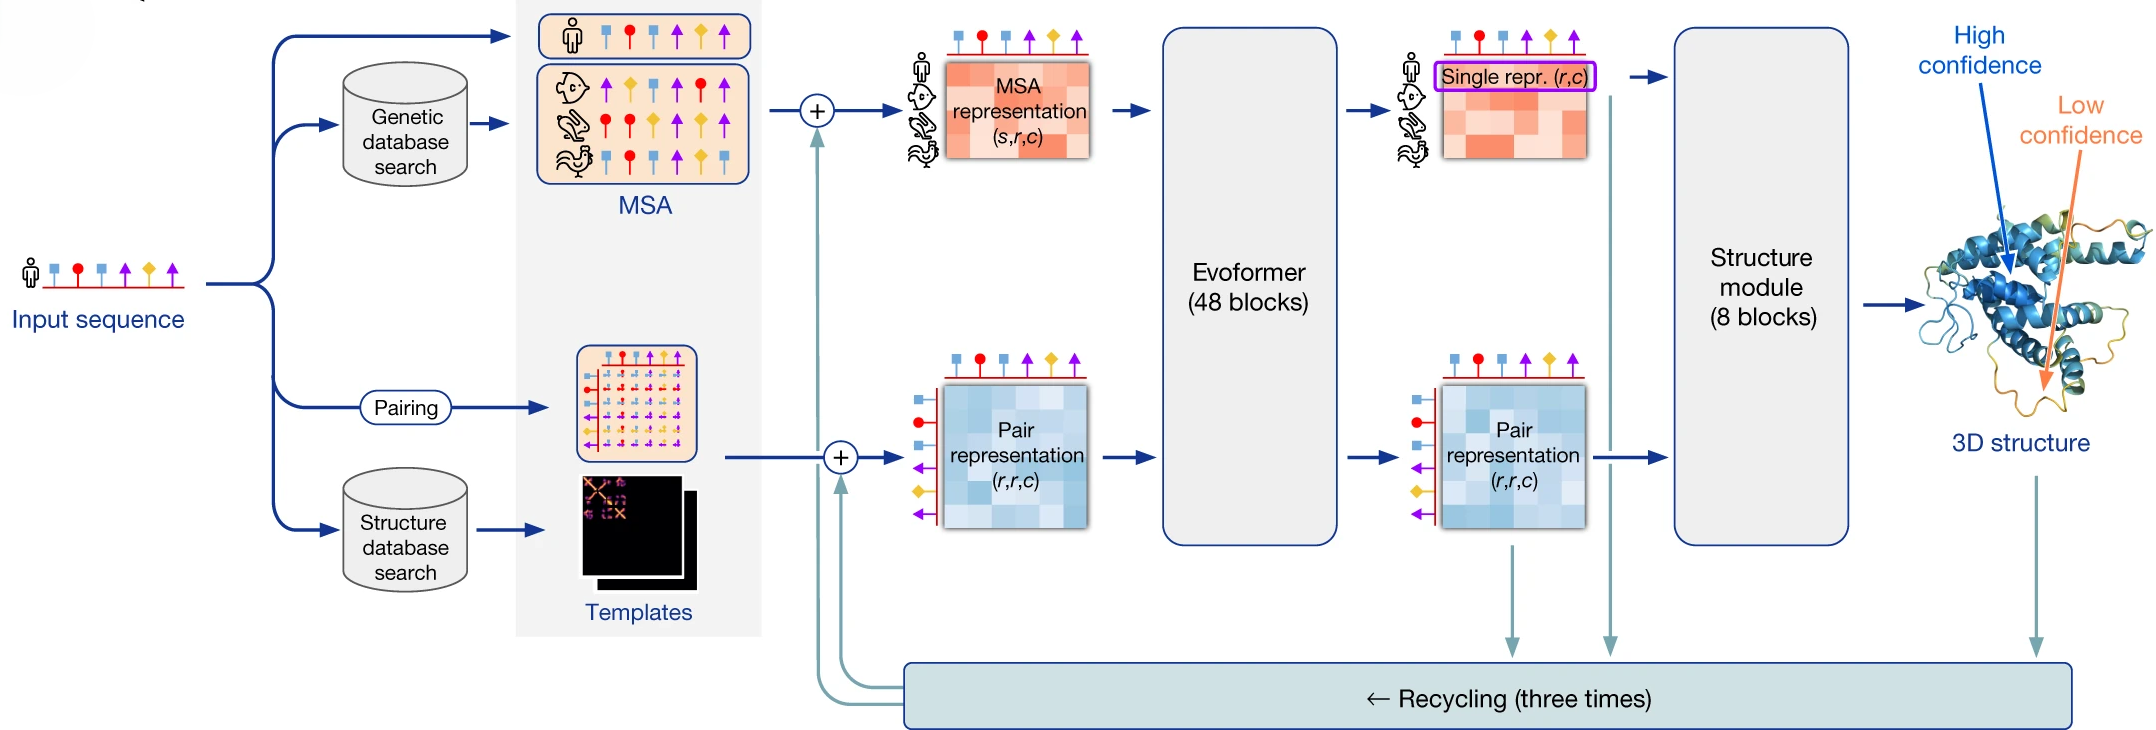
\includegraphics[width=1\linewidth]{figures/alphafold_pipeline.png}
    \caption{Schema semplificato della rete neurale di AlphaFold. Adattato e modificato dall'opera originale di Jumper et al. (2021), disponibile in Open Access sotto licenza Creative Commons Attribution 4.0 International (\url{http://creativecommons.org/licenses/by/4.0/}).}
    \label{fig:alphafold}
\end{figure}

Viene sfruttata un'architettura a rete neurale per integrare le nozioni chimico-fisiche e biologiche all'interno dell'insieme di regole di conformazione delle proteine.
Il modello si divide in due fasi principali:
\begin{enumerate}
    \item \textbf{Evoformer:} Primo modulo incaricato della previsione della struttura. Si approccia al problema computazionale interpretandolo come un \textbf{problema di inferenza di grafi} nello spazio tridimensionale. Tiene traccia degli amminoacidi propensi a mutare insieme, e a creare quindi strutture di avvolgimento complesse, tramite \textbf{Multiple Sequence Alignments} o \textbf{MSA}. Queste sono collezioni di sequenze di proteine omologhe allineate tra loro in un array bidimensionale, la cui analisi risulta utile per la previsone di coordinazioni tra amminoacidi e siti di ripiegamento proteico \cite{jumperHighlyAccurateProtein2021}.
    \item \textbf{Modello di Struttura:} Trasforma le informazioni ricavate dall'Evoformer in coordinate 3D reali. Ogni amminoacido è trattato come un corpo rigido indipendente, o "residue gas", che può ruotare e traslare nello spazio fino ad assumere la sua posizione "corretta" all'interno della conformazione della catena proteica.
    Viene usato un meccanismo di \textbf{Attenzione} (\textbf{Invariant Point Attentio, o IPA}) le cui iterazioni raffinano le informazioni spaziali degli elementi.
\end{enumerate}

AlphaFold non è un caso isolato. Nello stesso periodo, 
modelli di deep learning hanno identificato nuovi 
antibiotici attivi contro batteri resistenti 
\cite{stokesDeepLearningApproach2020}, permesso il 
"riposizionamento" di farmaci approvati durante 
la pandemia da COVID-19 \cite{richardsonBaricitinibPotentialTreatment2020}, 
e portato il primo farmaco interamente progettato da AI 
alla validazione clinica
\cite{xuGenerativeAIDiscoveredTNIK2025}. Questi risultati, 
che verranno discussi in dettaglio nel capitolo conclusivo, 
dimostrano come il ML applicato alla bioinformatica e in più particolare alla drug discovery sia già una realtà operativa nel campo della bioinformatica applicata alla \textit{drug discovery}.

\section{Obiettivi e Struttura dell'Elaborato}

Questo elaborato si propone di analizzare i principali 
metodi di Machine Learning e Deep Learning applicati 
alle fasi più critiche della pipeline farmaceutica, 
con particolare attenzione alla predizione delle 
interazioni farmaco-bersaglio e alla valutazione delle 
proprietà ADMET. 

La tesi studierà come la biologia molecolare e la farmacologia forniscano il 
contesto e il problema, mentre l'informatica (rappresentazione dei dati, architetture di apprendimento, 
ottimizzazione) fornisca gli strumenti e il linguaggio 
dell'analisi.

L'elaborato è organizzato come segue:

Il \textbf{Capitolo 2} introduce la pipeline di sviluppo 
farmaceutico, descrivendo le fasi principali del processo, dalla \textit{target identification} alla \textit{Lead Optimization} fino 
ai trial clinici, e il ruolo che l'AI svolge in ciascuna 
di esse. 
Vengono discussi l'attrition rate, il suo impatto 
economico e le cause principali del fallimento dei candidati 
farmaci.

Il \textbf{Capitolo 3} affronta il problema della 
rappresentazione molecolare, ovvero come tradurre entità 
biochimiche complesse, come molecole e proteine, in formati 
elaborabili da algoritmi di ML. 
Vengono analizzate le 
rappresentazioni lineari (SMILES, SELFIES), i fingerprint 
molecolari e le rappresentazioni a grafo.

Il \textbf{Capitolo 4} è il capitolo centrale dell'elaborato 
e tratta la predizione delle interazioni farmaco-bersaglio 
come problema computazionale formale. Dopo aver introdotto 
la formalizzazione matematica del problema DTI e DTA, 
vengono analizzate le metodologie di predizione, partendo dai 
metodi ligand-based e structure-based al docking 
molecolare, fino a trattare le architetture di Deep Learning 
più recenti: CNN, RNN, GNN e Transformer.

Il \textbf{Capitolo 5} tratta la valutazione delle 
proprietà ADMET, illustrando come il ML permetta di 
anticipare computazionalmente le cause più comuni di 
fallimento clinico, in particolare la tossicità molecolare, riducendo l'attrition rate 
nelle fasi avanzate della pipeline.
Verrà illustrata un'architettura multimodale d'esempio per ottimizzare la predizione e l'elaborazione delle conoscenze biochimiche, partendo dalle rappresentazioni dei farmaci candidati.

Il \textbf{Capitolo 6} presenta le conclusioni e 
sintetizza i contributi dei metodi analizzati,
documentando tre casi concreti di successo clinico (Baricitinib, Halicin e Rentosertib) che dimostrano il potenziale degli strumenti basati su AI 
nella drug discovery.
\chapter{Il pipeline di sviluppo farmaceutico}
%\begin{figure}[htbp]
    %\centering
    %\includegraphics[width=0.85\textwidth]{figures/pipeline.png}
    %TO-DO
   % \caption{Il pipeline di sviluppo farmaceutico.}
    %\label{fig:pipeline}
%\end{figure}
\section{Le fasi del Drug Development}

Lo sviluppo di un nuovo farmaco è un processo complesso e delicato, 
che si articola in più fasi sequenziali, ciascuna delle quali introduce 
vincoli tecnici, economici e regolatori che rendono l'intero percorso 
lungo, dispendioso e ad alto rischio di fallimento \cite{zhang2025}.

Negli ultimi due decenni si è distinta come principale strategia di discovery la \textbf{Target Based Drug Discovery} \cite{keshTargetBasedScreeningLead2023} (\textbf{TBDD}), processo che ha come inizio l'\textbf{identificazione del target}, 
ovvero la selezione di molecole biologiche, tipicamente  
proteine o acidi nucleici, la cui modulazione risulti rilevante 
per la malattia di interesse (ovvero target \textit{druggable}, trattabili farmalogicamente).
Si tratta del primo filtro a cui vengono sottoposte le molecole candidate ed è proprio il primo "collo di bottiglia" del processo di ricerca. 
Gli svariati approcci di screening utilizzati in questa fase di \textit{identification} possono essere classificati in quattro gruppi principali \cite{rasulTargetIdentificationApproaches2022}:
\begin{itemize}
    \item Approcci "diretti" o basati sull'\textbf{affinità} tra proteine e piccole molecole.
    \item Approcci basati sul \textbf{fenotipo}, usati per effettuare comparazioni tra i profili biologici delle molecole e quelli di farmaci già noti, di cui si conosce il comportamento.
    \item Approcci basati sull'individuazione dei \textbf{geni} specifici responsabili di farmacoresistenza da parte delle molecole.
    \item Approcci \textbf{computazionali}, in grado di fare previsioni sui target sulla base della complementarietà chimica dei candidati.
\end{itemize}
Sebbene molti di questi metodi, come l'\textit{affinity pull-down} e il \textit{whole-genome knockdow} siano ampiamente usati e rimangano i pilastri per la validazione dei target di interesse, questi presentano limiti intrinseci in termini di efficacia e costi. 
%----

Seguono le fasi di \textbf{drug discovery} vero e proprio, che si pongono l'obiettivo di identificare gli \textbf{\textit{hits}}, farmaci in grado di interagire con i target precedentemente individuati.
I geni candidati vengono espressi in grandi quantità in organismi poco complessi tramite la tecnologia del DNA ricombinante, permettendo lo \textbf{High-Throughput Screening} (HTS), ovvero uno screening ad alta velocità che agisce su vaste e variegate librerie chimiche \cite{keshTargetBasedScreeningLead2023}.

Sebbene l'HTS sia più performante in termini di costi rispetto ai metodi manuali, non si è dimostrato in grado di garantire la sicurezza o l'efficacia della molecola su organismi più complessi. 
Per superare tali limiti, emerge la necessità di tecniche di \textbf{Virtual Screening} (VS), che permettono di pre-selezionare \textit{in silico} i composti più promettenti, riducendo drasticamente il numero di test fisici necessari.

\subsection{Screening dei composti}
Il processo di screening rappresenta lo strumento per "setacciare" le librerie chimiche nella ricerca delle giuste interazioni biochimiche. Il \textbf{VS} si distingue dall'HTS per la sua capacità di andare oltre i limiti della ricerca fisica attuabile in laboratorio, valutando computazionalmente composti appartenenti a librerie fisiche o sintetizzabili su richiesta \cite{carlssonStructurebasedVirtualScreening2024}.
Questo approccio si divide in due macro-famiglie:
\begin{itemize}
    \item I metodi \textbf{ligand-based}, che si basano sull'ipotesi che molecole con proprietà simili a ligandi noti presentino attività biologica analoga. Tra questi, la \textbf{pharmacophore searching} identifica composti compatibili al target per caratteristiche chimico-spaziali (come la presenza di donatori e accettori di idrogeno o di gruppi aromatici in determinate posizioni) \cite{mcinnesVirtualScreeningStrategies2007a}.
    \item I metodi \textbf{structure-based}, che sfruttano la struttura tridimensionale del target tramite strumenti come il \textbf{molecular docking} o l'\textbf{ensemble docking}, quest'ultimo è un'evoluzione del primo che valuta il ligando su molteplici conformazioni del recettore, ottenendo così risultati più robusti rispetto all'approssimazione del recettore singolo e rigido.
\end{itemize}
Il virtual screening accelerato dal Machine Learning rappresenta una risposta al crescente e sempre più insostenibile peso computazionale del docking. Questo approccio prevede che un modello di ML venga addestrato sui risultati del docking su un sottoinsieme della libreria (si usano librerie dette "ultra-large") e che impari a predire i punteggi del docking per i composti incognita, senza eseguire il calcolo fisico. Questo approccio può portare a una riduzione di 100 volte il numero di composti da sottoporre a docking esplicito, mantenendo comunque un arricchimento dei composti top-scoring paragonabile allo screening esaustivo \cite{carlssonStructurebasedVirtualScreening2024}.


La \textit{hit discovery} è tuttavia solo il primo passaggio del processo di \textit{lead generation}, o \textit{Hit to Lead} (H2L), che si pone di valutare i composti individuati dalle \textit{hits} non solo per la loro presenza di attività, ma per la qualità della loro interazione con il target. 
In questa fase vengono analizzate potenza, selettività e proprietà fisico-chimiche di base, causando una scrematura che può apportare un miglioramento del legame chimico hit-target dell'ordine di grandezza nanomolare \cite{barcelosLeadOptimizationDrug2022}.
La fase finale di drug discovery è la \textit{Lead Optimization} (LO), che interviene per accentuare caratteristiche desiderate nei composti lead selezionati, o per correggere i difetti strutturali che impedirebbero ad essi di superare i trial clinici.
La LO moderna è un processo razionale guidato da metodi computazionali che includono studi farmacoforici, docking molecolare (metodo utilizzato per prevedere l'orientamento di un ligando su un recettore per la formazione di un complesso stabile), dinamica molecolare (simulazioni con lo scopo di ottenere dati sulle proprietà fisico-strutturali delle molecole) e QSAR. 
In paricolare, il \textbf{QSAR} (Quantitative Structure-Activity Relationship) rappresenta un approccio di modellazione statistica volto a correlare le caratteristiche strutturali con l'attività biologica dei composti, evolvendosi oggi in modelli di Machine Learning capaci di interpretare e prevedere queste caratteristiche per generare risultati nuovi \cite{barcelosLeadOptimizationDrug2022}.

Una volta ottenute le lead ottimizzate si può passare agli \textbf{studi pre-clinici}, condotti su modelli animali per valutare 
sicurezza ed efficacia dei farmaci, prima che questi vengano testati sull'essere umano. 
La fase successiva, quella degli effettivi \textbf{trial clinici}, si 
articola a sua volta in tre stadi progressivi: 
\begin{itemize}
    \item La fase~I verifica la 
sicurezza del composto su un piccolo gruppo di soggetti sani;
    \item La fase~II ne valuta l'efficacia su pazienti affetti dalla patologia interessata;
    \item La fase~III, condotta su popolazioni più ampie, 
costituisce il test definitivo richiesto per l'approvazione regolatoria. 
\end{itemize}  
Al termine di questo percorso, il farmaco approvato entra nella fase 
di \textbf{post-market surveillance}, in cui vengono monitorati nel 
lungo periodo gli effetti collaterali e la stabilità della formulazione.

\section{Attrition Rate e impatto economico}
Il percorso che racchiude queste fasi è caratterizzato da un problema fondamentale: nonostante l'accelerazione in ambito tecnologico degli ultimi anni e la comparsa di nuovi strumenti computazionali ad ausilio del processo, il successo delle fasi cliniche rimane un obiettivo estremamente difficile da raggiungere. Questo fenomeno è descritto dall'\textbf{attrition rate}, ovvero il tasso di riduzione ("logoramento") del numero di candidati farmaci durante l'avanzamento della pipeline.
Delle migliaia di molecole potenziali individuate dalla prima fase di discovery, solo una piccola frazione sopravvive ai test clinici e meno del 10\% dei composti che entrano nel primo step di trial raggiunge l'approvazione finale dalle autorità regolatorie.

Questo elevato tasso di insuccesso si traduce in elevatissimi costi economici.
Lo sviluppo di un nuovo farmaco richiede oggi un investimento medio di circa 
\textbf{2,6 miliardi di dollari americani} e un arco temporale compreso tra 
i dodici e i quindici anni \cite{zhang2025}. 
Inoltre, anche il ritorno economico per le industrie farmaceutiche 
è drasticamente calato: nell'arco di un decennio, per ogni dollaro 
investito in ricerca il ritorno economico è crollato drasticamente, passando da 10 a meno di 2 centesimi 
\cite{freedmanHuntingNewDrugs}.

Le cause di questo elevato tasso di fallimento sono molteplici. 
In primo luogo, molti farmaci per malattie comuni e con meccanismi biologici noti sono già stati scoperti; ciò che rimane da 
esplorare riguarda patologie più rare e complesse, dove l'identificazione 
di molecole target risulta più difficile \cite{freedmanHuntingNewDrugs}. 
Inoltre, la selezione delle molecole nelle fasi di \textit{discovery} può essere basata su parametri toppo semplici e poco esaustivi. Infatti, come evidenziato da \textbf{Kenakin} \cite{kenakinKnowYourMolecule2024}, la mancanza di efficacia clinica e i problemi di sicurezza legati alla tossicità rimangono le cause primarie del logoramento dei candidati farmaci, ed entrambi sono imputabili a una descrizione farmacologica superficiale e poco approfondita dei \textbf{lead} stessi.

\section{Il ruolo dell'AI nella pipeline}
L'integrazione dell'Intelligenza Artificiale (AI) e del Deep Learning (DL)
ha trasformato la pipeline di ricerca farmaceutica da un processo basato su "trial and error" a una percorso più disciplinato, guidato dalla raccolta e dall'analisi dei dati biologici \cite{zhang2025}.
Questi strumenti vengono impiegati trasversalmente, in ciascuna delle diverse fasi più delicate e "logoranti" del processo.

Nella fase di \textbf{target identification}, l'AI sta affiancando 
e in alcuni casi sostituendo i metodi tradizionali di screening, 
prima basati sull'analisi dettagliata dell'affinità tra molecole. 
Il nuovo approccio consiste nel rappresentare i geni per la loro \textit{funzione biologica}, analogamente alle 
tecniche di \textit{word embedding} sviluppate nel Natural Language Processing (NLP). 
Negli step successivi dello sviluppo del composto, il contributo più significativo si osserva nella predizione dei comportamenti di interazione farmaco-proteina (DPI).
Queste stime sono solitamente compiute su uno spazio chimico di scala molto ampia, e richiedono l'analisi di molte interazioni ancora sconosciute. Proprio per questo, i modelli di Machine Learning vengono addestrati in modalità semi-supervisionato per etichettare queste interazioni incognite, integrando efficacemente informazioni eterogenee, quali la struttura chimica del composto, i dati genomici e le reti di interazione.
L'importanza di affinare tali modelli risiede nella necessità di colmare il \textit{knowledge gap} relativo agli effetti collaterali:
è stato infatti stimato che circa 1.000 proteine umane siano potenzialmente responsabili di tossicità \textit{off-target}. 

Identificare precocemente queste interazioni impreviste risulta dunque fondamentale per prevedere e mitigare interazioni nocive già nelle fasi preliminari dello sviluppo in silico \cite{dara2022}.


\chapter{Rappresentazione molecolare e machine readability}

\section{Lettura di dati chimici e biologici in informatica}
L'applicazione di tecniche di Intelligenza Artificiale nell'ambito biochimico richiede il passaggio fondamentale da dati chimici a dati computazionali. Questi ultimi non devono essere semplicemente informazioni biologiche tradotte digitalmente, ma devono essere presentate in formati effettivamente elaborabili da algoritmi e tecnologie di ML \cite{jablonkaMakingCollectiveKnowledge2022}.\\
Storicamente, i risultati venivano registrati in forma cartacea, portando alla perdita di una vasta mole di dati non pubblicati.
Al giorno d'oggi, invece, sebbene la quasi totalità degli strumenti di laboratorio sia in grado di rappresentare e salvare i dati in formato digitale (e accessibile ad altri ricercatori), una parte significativa di questi resta in formati analogici o non accessibili automaticamente dagli agenti computazionali.\\
Risulta quindi necessaria, per sopperire a questa frammentazione di dati, una transizione verso una scienza più aperta, che integri l'implementazione di dati \textit{machine-actionable}, ovvero adatti all'automatizzazione computazionale.\\
In questo contesto, la rappresentazione molecolare deve raggiungere un \textit{trade-off} tra completezza informativa e complessità. 
Infatti, sebbene formati altamente strutturati, in grado di descrivere esaustivamente le proprietà chimiche, geometriche e funzionali delle molecole, si siano dimostrati ideali per modelli di ML, questi possono risultare estremamente onerosi per il lavoro dei chimici in laboratorio.\\
Senza una rappresentazione standardizzata che rispetti i principi \textbf{FAIR} (\textit{Findable, Accessible, Interoperable, Reusable}), l'efficacia dei modelli di Machine Learning e Deep Learning nella previsione delle proprietà molecolari risulterebbe limitata dalla qualità del dato in ingresso \cite{jablonkaMakingCollectiveKnowledge2022}.
\begin{figure}
    \centering
    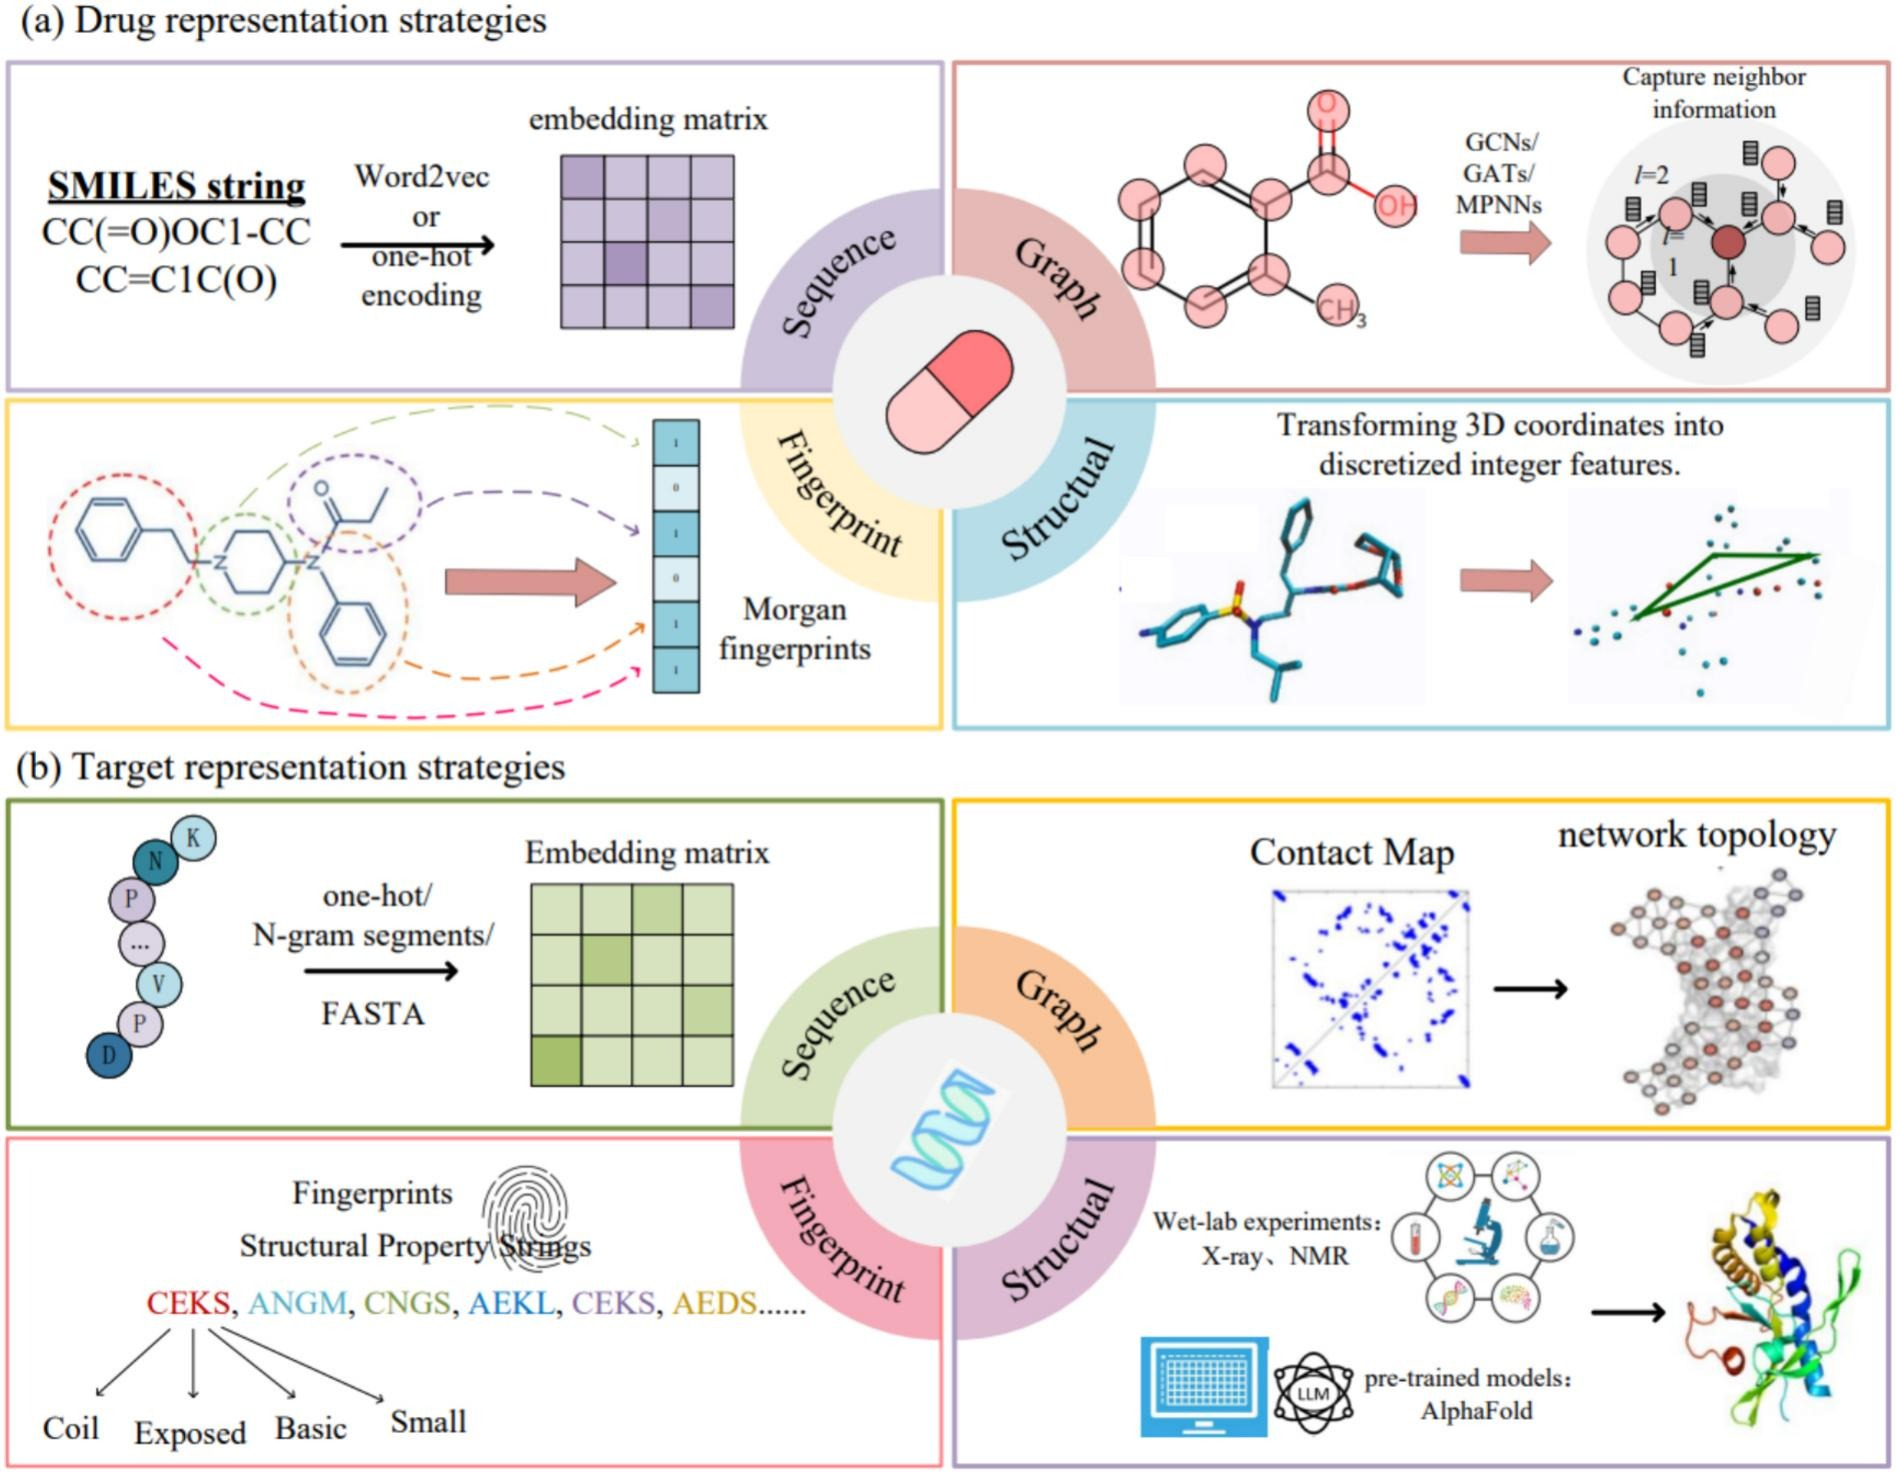
\includegraphics[width=0.75\linewidth]{figures/rappresentazioni_wang.png}
    \caption{Strategie di rappresentazione per molecole farmacologiche e proteine bersaglio. (a) Rappresentazione dei composti chimici tramite SMILES, grafi molecolari, fingerprint (Morgan) e caratteristiche strutturali 3D. \\(b) Rappresentazione dei target biologici tramite sequenze FASTA, descrittori strutturali e modelli predittivi (es. AlphaFold). Figura riprodotta con il permesso di Elsevier, da Wang et al., A unified survey on drug-target interaction and binding affinity prediction: Models, representations, and challenges", Biotechnology Advances, 2026. Licenza numero: 6286991125834.}
    \label{fig:rappresentazioni_wang}
\end{figure}
\clearpage
\section{Rappresentazioni lineari: SMILES e SELFIES}
La necessità di disporre di dati FAIR e \textit{machine readable/actionable} ha portato allo sviluppo di diverse metodologie di codifica di dati chimici in formati meno complessi, processabili da algoritmi e metodi di machine learning.
\subsection{SMILES}
Il sistema \textbf{SMILES} (Simplified Molecular-Input Line-Entry System) rappresenta lo standard moderno più diffuso per la rappresentazione di molecole chimiche nell'ambito delle applicazioni di intelligienza artificiale.\\
Si basa sulla descrizione delle strutture chimiche attraverso stringhe di caratteri alfanumerici ASCII \cite{aksamitHybridFragmentSMILESTokenization2024}, sottoponibili a processi NLP.
Una stringa SMILES rappresenta la molecola come una catena di atomi, dove le ramificazioni sono indicate tra parentesi tonde, le chiusure degli anelli da numeri corrispondenti (per esempio, 1 con 1, ecc...), i simboli "-", "=", "\#" \cite{sadeghiCanLargeLanguage2024} rappresentano diversi tipi di legame, mentre "@", "/", "\textbackslash" diverse conformazioni isomeriche \cite{aksamitHybridFragmentSMILESTokenization2024}.
$$CC(C)(C)C(=O)C(N1C=CN=C1)OC2=CC=C(C=C2)Cl$$
\begin{figure}[htbp]
    \centering
    \chemfig{C(-[::90]C)(-[::-90]C)(-[::180]C)-C(=[::90]O)-C(-[::90]N*5(-CH=N-CH=CH-))-O-P*6(-CH=CH-C(Cl)=CH-CH=)}
    \caption{Rappresentazione SMILES e struttura molecolare del Climbazolo.}
    \label{fig:climbazolo_smiles}
\end{figure}
\begin{figure}[h]
    \centering
    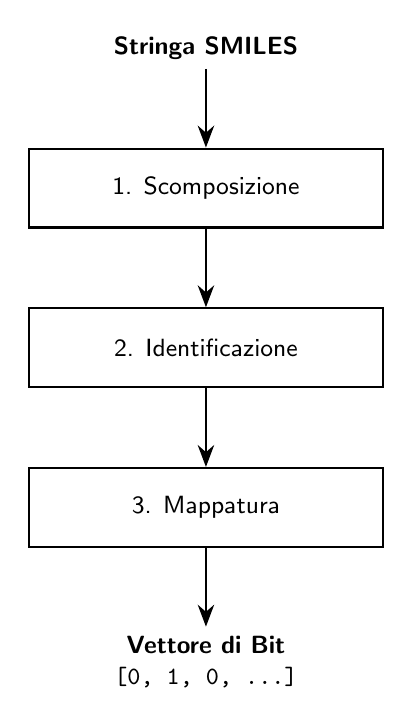
\begin{tikzpicture}[
        block/.style={
            rectangle, 
            draw=black, 
            thick, 
            minimum width=4.5cm, 
            minimum height=1cm, 
            align=center,
            font=\small\sffamily
        },
        textnode/.style={
            font=\small\sffamily\bfseries,
            align=center
        },
        arrow/.style={
            -{Stealth[scale=1.2]}, 
            thick
        },
        node distance=1.0cm
    ]

        \node[textnode] (smiles) {Stringa SMILES};
        
        \node[block, below=of smiles] (scomp) {1. Scomposizione};
        
        \node[block, below=of scomp] (ident) {2. Identificazione};
        
        \node[block, below=of ident] (mapp) {3. Mappatura};
        
        \node[textnode, below=of mapp] (bits) {Vettore di Bit \\ \normalfont\ttfamily[0, 1, 0, ...]};
        \draw[arrow] (smiles) -- (scomp);
        \draw[arrow] (scomp)  -- (ident);
        \draw[arrow] (ident)  -- (mapp);
        \draw[arrow] (mapp)   -- (bits);

    \end{tikzpicture}
    \caption{Flusso del processo di trasformazione chimico-digitale da stringa SMILES a vettore di bit.}
    \label{fig:smiles_to_bits_vertical}
\end{figure}
Le SMILES vengono tradotte in bit tramite \textit{processing} a Fingerprint Molecolari:
Le stringhe entrano in input per passare in una prima \textbf{Fase di Scomposizione}, da cui si ottengono frammenti di natura diversa in base all'algoritmo usato (possono essere percorsi tra atomi, aree di intorno circolare, ecc...) \cite{boldiniEffectivenessMolecularFingerprints2024}.\\
Segue poi la fase di \textbf{Encoding}, in cui ogni frammento riceve un identificatore numerico basato sulle proprietà atomiche.\\
Infine la fase di \textbf{Hashing}, dove gli identificatori vengono mappati in un vettore di bit a dimensione fissa, tramite funzioni apposite.\\  
Nonostante la sua ampia diffusione, \textbf{SMILES} presenta criticità strutturali che ne limitano l'efficacia:
\begin{itemize}
    \item Un primo limite della rappresentazione risiede nella \textbf{mancanza di univocità} che rende possibile la descrizione di una stessa molecola da molteplici stringhe diverse \cite{leonComparingSMILESSELFIES2024}.
    \item Inoltre, il sistema SMILES è soggetto a una notevole fragilità sintattica che può portare facilmente all'invalidazione delle stringe a causa di piccole mutazioni di caratteri singoli (come una parentesi non chiusa), che rendono il complesso privo di significato biologico. 
    Questa vulnerabilità risulta particolarmente problematica nell'uso di \textbf{Language Model} e modelli generativi, i quali producono combinazioni casuali di simboli durante la campionatura dello spazio latente.
    \item Infine, la natura lineare delle stringhe non premette di raffigurare correttamente la conformazione tridimensionale della molecola e le sue complesse relazioni spaziali \cite{ucakReconstructionLosslessMolecular2023}.
\end{itemize}
\subsection{SELFIES}
Le stringhe \textbf{SELFIES} (SELF-referencing Embedded Strings) sono state progettate con lo scopo di superare i limiti di SMILES, garantendo una robustezza del 100\% \cite{krennSELFIESFutureMolecular2022} ed eliminando gli errori sintattici derivati dalle variazioni di caratteri.
Ogni stringa SELFIES valida corrisponde a una molecola valida, poiché la notazione si basa su una mappatura che impedisce violazioni dei vincoli fisici e strutturali. 
A differenza di SMILES, che è una notazione descrittiva, SELFIES è più simile a una libreria di stati finiti, i quali compongono una grammatica formale, un \textbf{automa} \cite{leonComparingSMILESSELFIES2024}.\\
I SELFIES sono racchiusi tra parentesi quadre e definiscono, tramite identificatori locali, le ramificazioni e gli anelli in un unico punto, specificandone la lunghezza tramite \textit{overloading}:\\
Quando il modello incontra un token di ramificazione o di anello, i numeri immediatamente successivi vengono interpretati come dimensione della sottostruttura di riferimento \cite{leonComparingSMILESSELFIES2024}.
In questo modo vengono evitate con successo variazioni indesiderate causate da riferimenti con indici lontani tra loro nella stringa. \\
Questa prorpietà rende i SELFIES particolarmente adatti per l'impiego in modelli generativi, poiché l'intero spazio latente esplorato da questi sarebbe composto da strutture chimicamente valide, che non richiederebbero ulteriori filtri o controlli. 
\begin{figure}[htbp]
    \centering
    $$C1=CC=CC=C1$$
    $$[C][=C][C][=C][C][=C][Ring_1][=Branch_1]$$
    \caption{Confronto tra le notazioni per il benzene: SMILES (sopra) e SELFIES (sotto) \cite{krennSELFIESFutureMolecular2022}.}
    \label{fig:smiles_vs_selfies}
\end{figure}
Nonostante i vantaggi tecnici offerti dalle stringhe SELFIES in termini di robustezza, il sistema \textbf{SMILES} rimane comunque lo standard cheminformatico più popolare per diverse ragioni:\\
In particolare, la sintassi SELFIES e il suo meccanismo di overloading dei token risultano più difficili da interpretare visivamente e meno intuitivi per gli operatori umani \cite{leonComparingSMILESSELFIES2024}.
Inoltre, sorprendentemente, in alcuni task di classificazione, modelli basati su SMILES hanno mostrato di superare le controparti basate su SELFIES. Questo comportamento può essere dovuto al fatto che le SMILES, essendo più sensibili alla tokenizzazione (generano sequenze di token più brevi ed efficienti per la stessa molecola), permettono di catturare pattern unici, talvolta trascurati dai modelli SELFIES, che tendono invece a generalizzare eccessivamente le caratteristiche molecolari.\\
Questa maggiore compattezza permette ad architetture come i \textbf{Transformer} di allocare la matrice di \textbf{attention} in modo più efficace, concentrandosi su un numero minore di unità informative \cite{leonComparingSMILESSELFIES2024}.\\
\section{Fingerprint molecolari}
I \textit{fingerprint} d'altro canto adottano un approccio vettoriale:\\
Come citato prima, la molecola viene decomposta in frammenti locali che vengono poi convertiti, tramite funzioni di hashing, in un formato \textit{machine-readable}, ovvero in un vettore numerico di lunghezza fissa (di solito pari a 1024 bit).
Questi vettori codificano caratteristiche specifiche, come la presenza o l'assenza di determinate strutture (\textit{binary fingerprints}) o il numero di occorrenze di determinati pattern molecolari (\textit{count-based fingerprints}), permettendo agli algoritmi di ML di analizzare facilmente le molecole per task di \textit{Virtual Screening} e previsione di proprietà biologiche \cite{boldiniEffectivenessMolecularFingerprints2024}.\\
Esistono diverse categorie principali di fingerprint, suddivise in base al tipo di informazione che catturano \cite{boldiniEffectivenessMolecularFingerprints2024}:
\begin{itemize}
    \item Fingerprints "\textbf{String-based"}: Operano direttamente sulla stringa SMILES, frammentando la stringa in sottosequenze di dimensione fissa e calcolando il numero di occorrenze di questi frammenti.
    \item Fingerprints "\textbf{Path-based"}: Data una rappresentazione molecolare \textbf{a grafo} (che verrà approfondita nella prossima sezione), vengono analizzati i \textbf{cammini lineari}, utilizzando, ad esempio, algoritmi come il \textbf{DFS (Depth First Search)}, che percorrono la molecola partendo da ogni singolo atomo fino ad una distanza di \textit{d} legami, mantenendo un record di ogni percorso unico.
    \item Fingerprints \textbf{Farmacoforici}: Si focalizzano sulla reattività chimica piuttosto che sulla struttura. I farmacofori sono l'insieme di caratteristiche chiave di una molecola all'interno del suo ambiente biochimico, come i punti di interazione, donatori/accettori, legami a idrogeno, gruppi idrofobici, ecc...
    Questi fingerprints codificano il modo in cui la molecola interagisce con l'ambiente circostante, concentrandosi maggiormente sulle proprietà funzionali, piuttosto che sulla struttura anatomica esatta.
    \item Fingerprints "\textbf{Substructure-based}": Basati sulla presenza di sottostrutture chimiche predefinite. Questo tipo di fingerprints utilizza un "dizionario" di frammenti noti, precedentemente individuati da esperti.
    \item Fingerprints \textbf{Circolari}: Partendo da un atomo, l'algoritmo di fingerptint aggrega le informazioni degli atomi vicini tra loro entro un raggio crescente, di fatto scomponendo la molecola in frammenti sullo stesso arco.
    Si tratta della tecnica più utilizzata per i modelli di Machine Learning, poiché è in grado di catturare informazioni sull'ambiente locale dell'atomo in modo strutturato ed esaustivo.
\end{itemize}
\subsection{Esempi di fingerprints}
Alcuni esempi appartenenti alla categoria di rappresentazione con \textbf{fingerprint molecolari} sono le \textbf{Morgan fingerprints} (o \textit{Extended Connectivity Fingerprints} (ECFP)) e le \textbf{MACCS key}.\\
Le prime si distinguono come strumento fondamentale e standard \textit{de facto} per la codifica dei composti farmaceutici \textit{drug-like}. 
\\Queste fingerprints \textbf{circolari}, con lunghezza pari a $1024$ bit, sono in grado di costruire dinamicamente i frammenti delle sottostrutture molecolari, a partire dalla loro rappresentazione a grafo \cite{boldiniEffectivenessMolecularFingerprints2024}.\\
Le \textbf{MACCS key (Molecular Access System)}, invece, si basano su un approccio più storico e utilizzano, come suggerito dal nome, un \textbf{dizionario} statico predefinito di sottostrutture, da cui attingere per codificare le strutture:\\
Sono rappresentate da un vettore binario da \textbf{166} bit di lunghezza. Ognuno di questi bit codifica la assenza/presenza ({0,1}) di una specifica caratteristica strutturale, definita tramite i pattern \textbf{SMARTS} (SMILES Arbitrary Target 
Specification) \cite{boldiniEffectivenessMolecularFingerprints2024} \cite{ucakReconstructionLosslessMolecular2023} che identificano, all'interno del dizionario, frammenti, gruppi funzionali o motivi molecolari.
\begin{lstlisting}[language=Python, caption={Estrazione delle MACCS Keys tramite RDKit}, label={lst:maccs_code}]
    from rdkit import Chem
    from rdkit.Chem import MACCSkeys

    smiles = "CC(C)Cc1ccc(cc1)C(C)C(=O)O"
    mol = Chem.MolFromSmiles(smiles)
    maccs_key = MACCSkeys.GenMACCSKeys(mol)
    bit_string = maccs_key.ToBitString()

    maccs_166 = [int(b) for b in bit_string][1:]
\end{lstlisting}
\begin{figure}
    \centering
    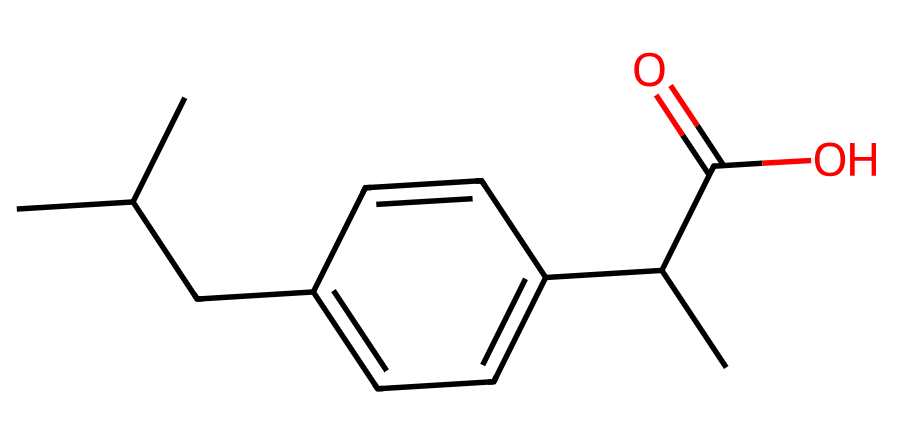
\includegraphics[width=0.5\linewidth]{figures/svgIbuprofene.png}
    \caption{Struttura chimica dell'Ibuprofene. \\Indici dei bit attivi rilevati: [74, 115, 123, 139, 141, 149, 154, 155, 157, 159, 160, 162, 163, 164, 165]}
\end{figure}
\begin{figure}
    \centering
    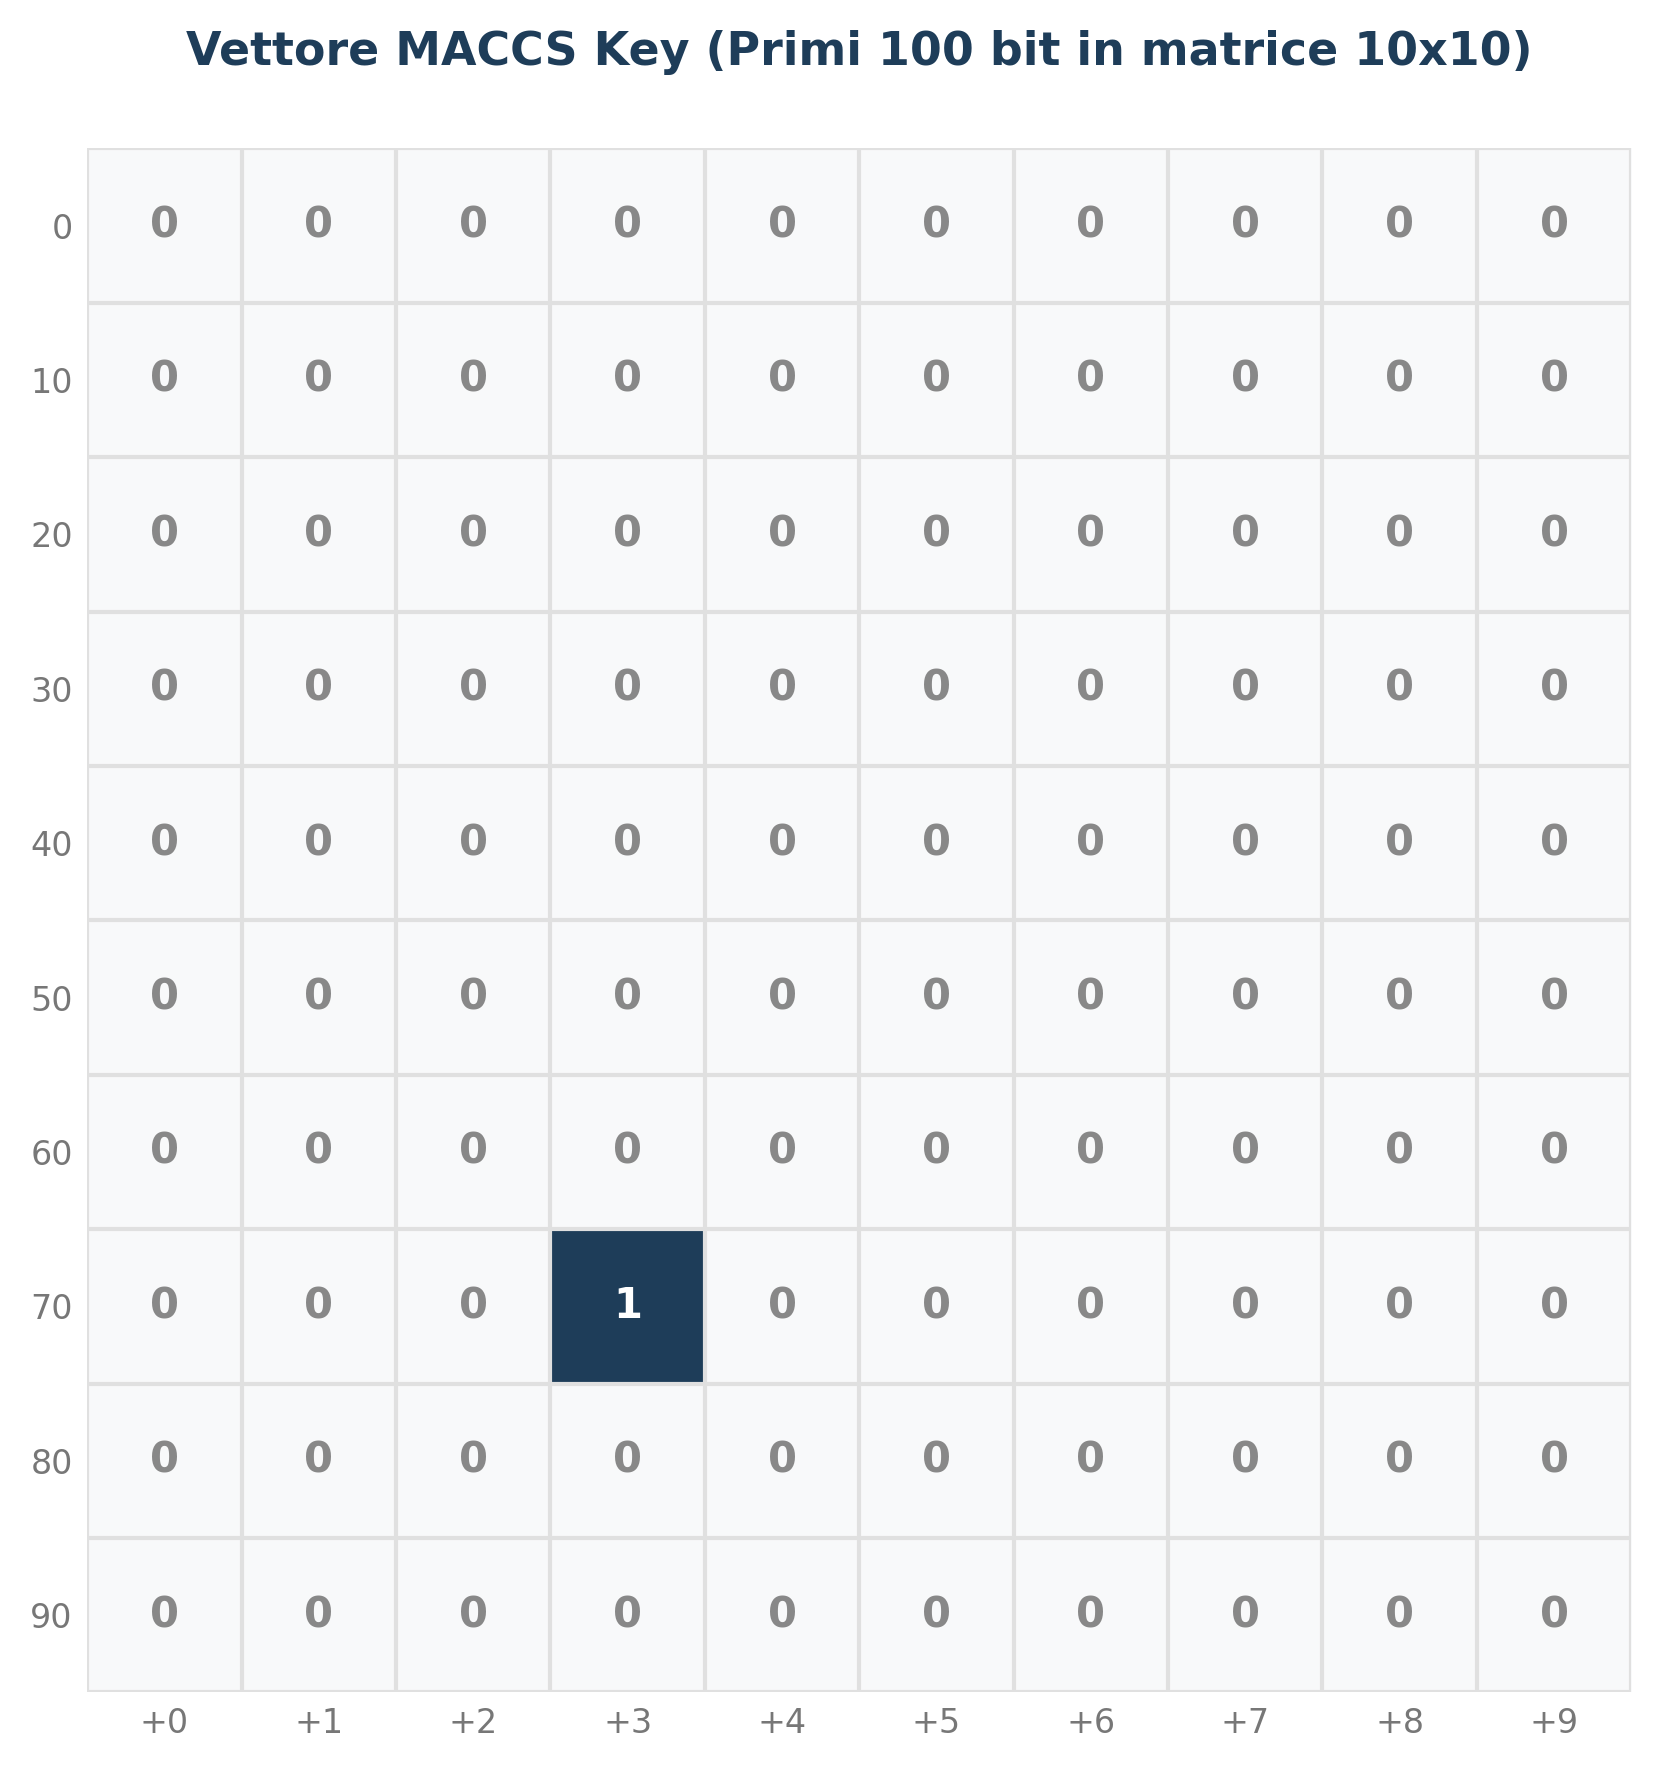
\includegraphics[width=0.4\linewidth]{figures/vettore_maccs_ibu.png}
    \caption{Primi 100 bit del fingerprint dell'Ibuprofene}
\end{figure}
Nonostante i fingerprint molecolari offrano diversi vantaggi significativi rispetto alle rappresentazioni lineari, specialmente in termini di efficienza computazionale e interpretabilità, questi presentano una perdita di informazioni non trascurabile durante il loro processo di codifica \textit{hashing}, soprattutto per quanto riguarda i dati sulla connettività dei frammenti \cite{ucakReconstructionLosslessMolecular2023}.
È quindi necessario risalire a una \textbf{ricostruzione lossless} (senza perdita di informazioni), invertendo la traduzione dei fingerprint.
Si tratta di un processo computazionale basato sull'architettura \textbf{Transformer}, che viene utilizzata come un sistema di traduzione in grado di apprendere le dipendenze globali tra input (i bit del fingerprint) e output (token di stringhe molecolari molecolare), grazie al meccanismo di \textit{multi-head attention}.
Il modello riesce quindi a decodificare i fingerprint strutturali riconducendoli a rappresentazioni lineari (SMILES o SELFIES) \cite{ucakReconstructionLosslessMolecular2023}.\\
\section{Rappresentazione a grafo}
La rappresentazione a \textbf{grafo} contituisce l'approccio più intuitivo e fedele alla realtà fisica per la digitalizzazione delle strutture chimiche, superando i limiti informativi delle notazioni lineari e minimizzando la perdita di dati.\\
La molecola viene rappresentata come un grafo non orientato  $G=(V,E)$ \cite{wangGraphNeuralNetworks2023}, in cui:
\begin{description}
    \item[$V$ (Nodi):] Rappresentano gli atomi della molecola. 
    \item[$E$ (Archi):] Rappresentano i legami chimici interatomici.
\end{description}
Tale struttura permette di codificare direttamente la topologia (informazioni bidimensionali, come i legami covalenti) e la connettività della molecola (la geometria, le informazioni tridimensionali), trasformando le proprietà del composto in \textbf{matrici} elaborabili da modelli di Intelligenza Artificiale.\\
Per essere interpretata dai computer, la struttura del grafo viene convertita in matrici, convertendo così la informazioni chimiche in un linguaggio matematico adatto ad essere appreso dai modelli \cite{wangGraphNeuralNetworks2025}.\\
Questa rappresentazione è il pilastro fondamentale per le \textbf{GNN (Graph Neural Networks)}, argomento che verrà affrontato nel prossimo capitolo.
\begin{figure}
    \centering
    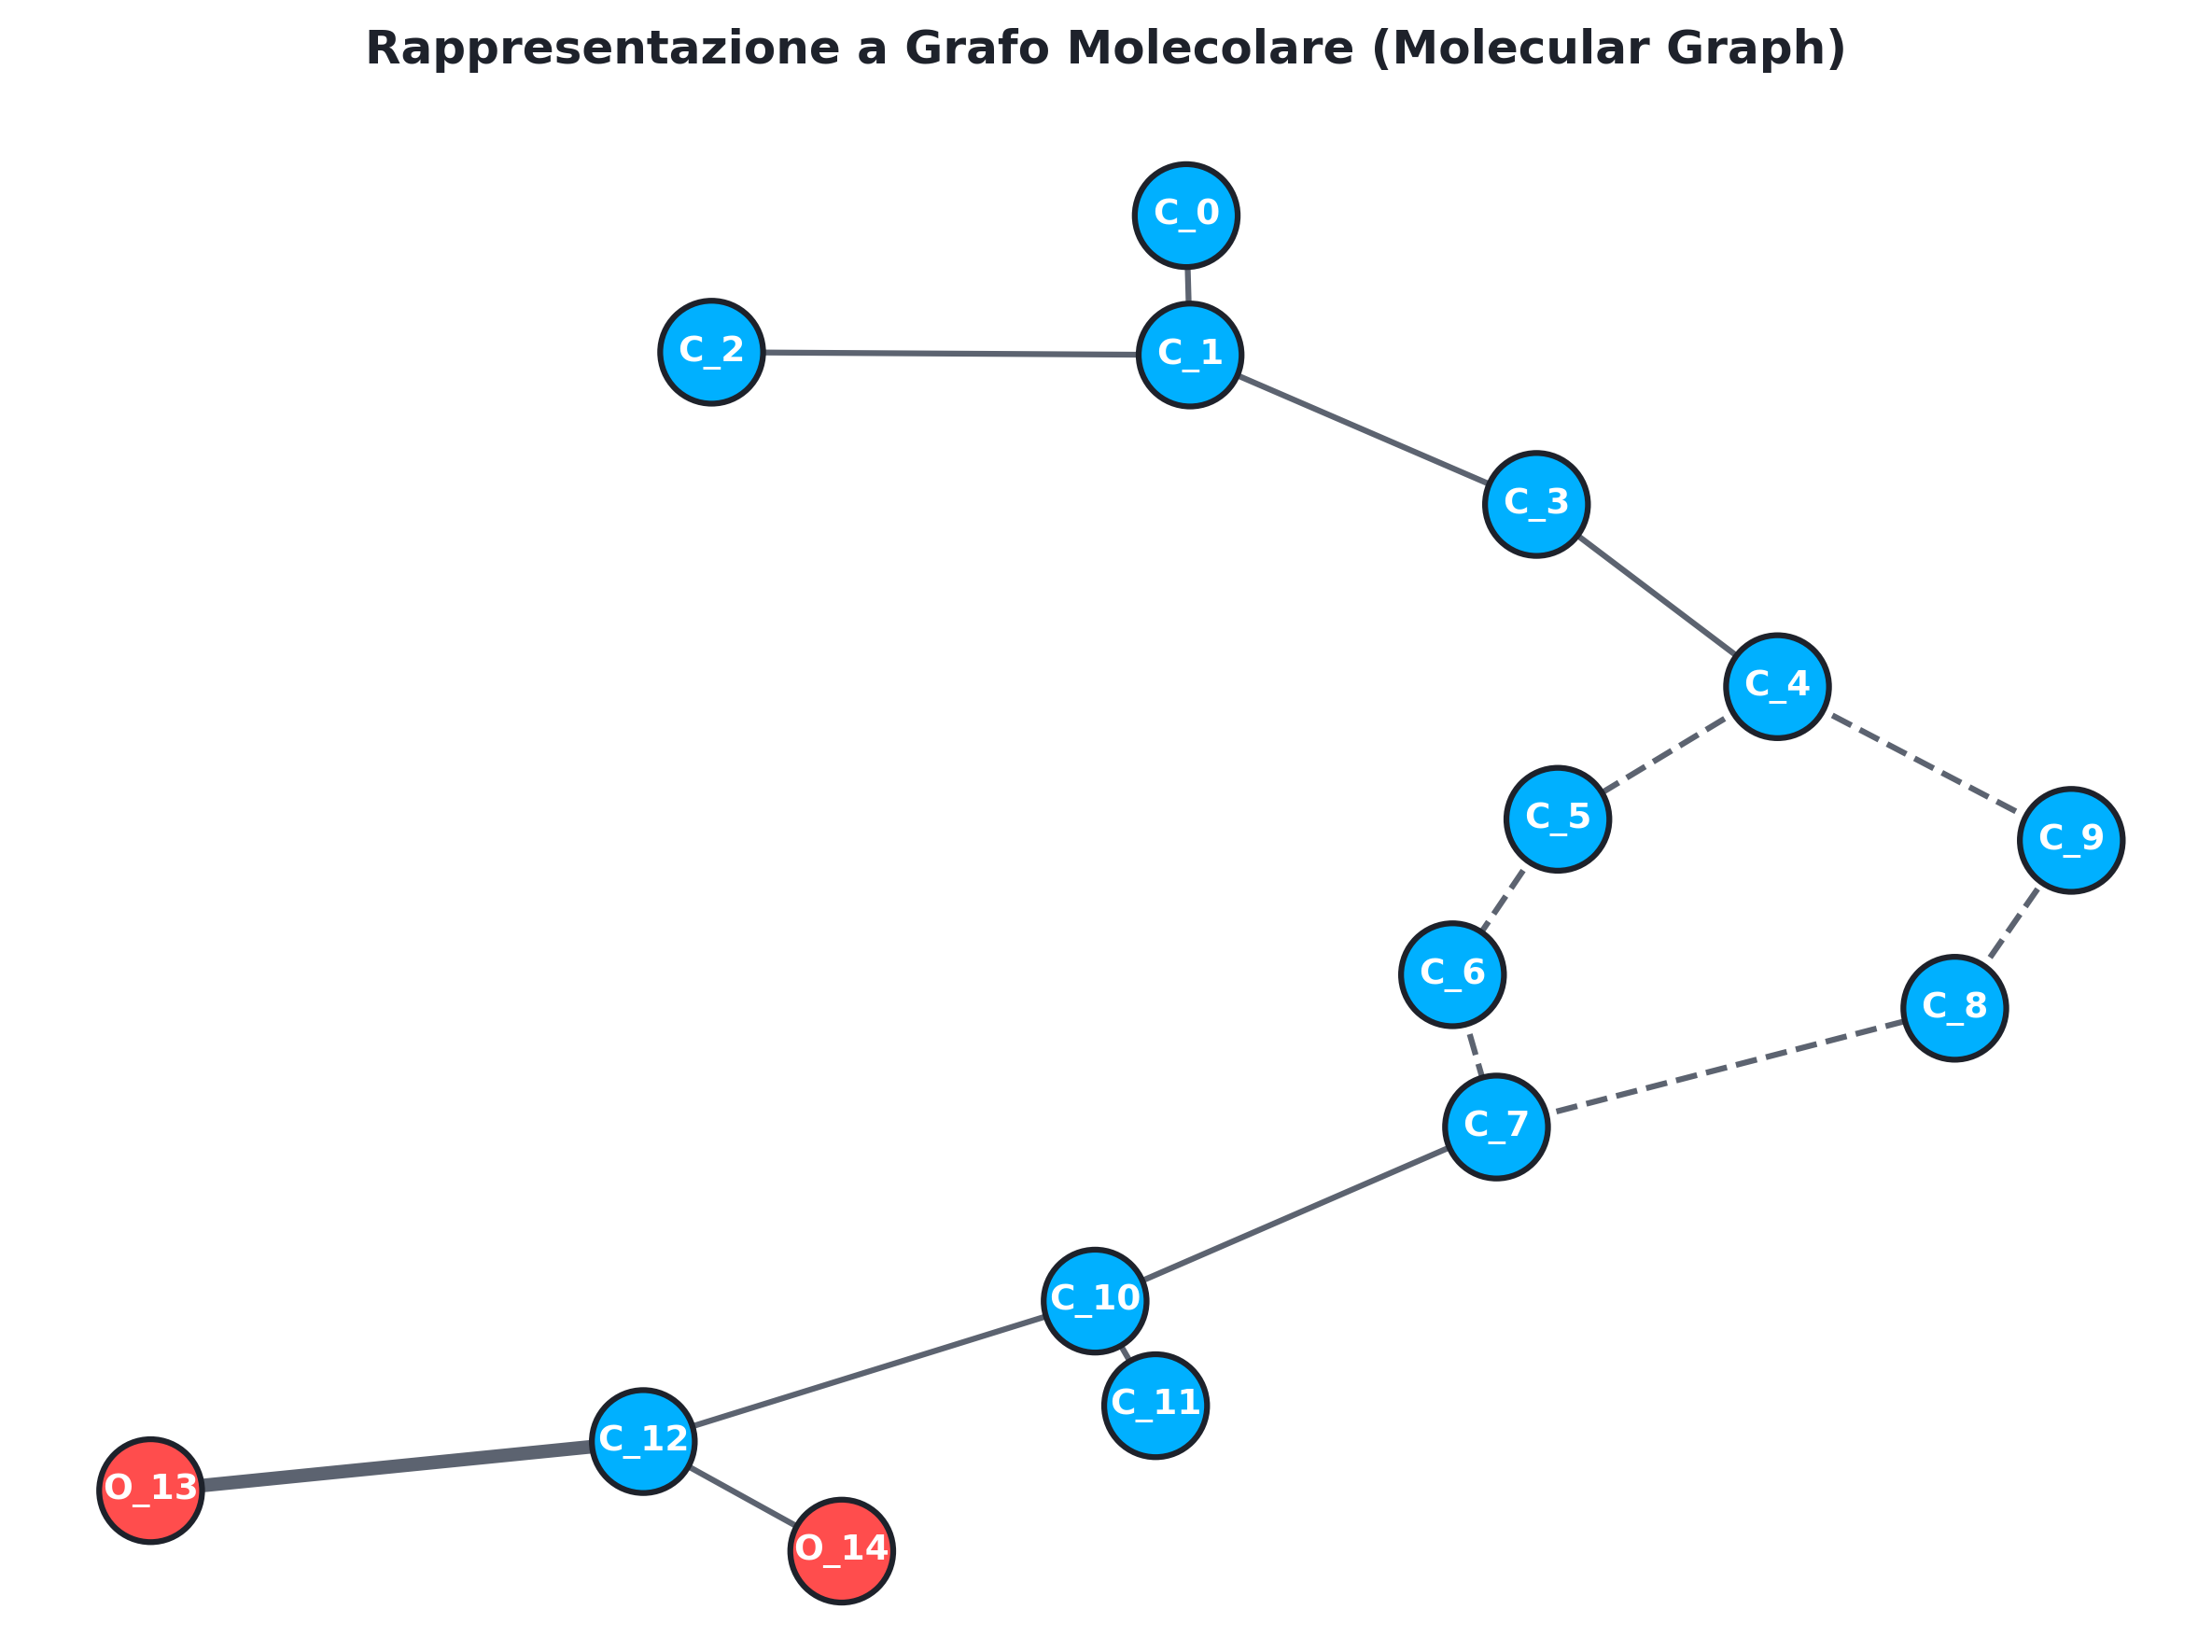
\includegraphics[width=0.75\linewidth]{figures/molecular_graph_ibu.png}
    \caption{Rappresentazione topologica non orientata $G = (V, E)$ dell'Ibuprofene generata da codice grazie a librerie RDKit e NetworkX.}
    \label{fig:graph}
\end{figure}
\clearpage
\section{Embedding molecolari e modelli pre-addestrati}
L'\textbf{embedding molecolare} è un'operazione fondamentale nella ricerca farmaceutica.
Questo processo consiste nel trasformare le informazioni relative al contesto strutturale e chimico di una molecola in una \textbf{rappresentazione numerica}, tipicamente sotto forma di vettori densi ad alta dimensione.\\
Questa pratica si basa sulla seguente ipotesi: \textbf{tutte le molecole strutturalmente simili, presentano comportamenti e proprietà altrettanto simili}.  Seguendo questa ipotesi, l'embeddig cerca di mappare queste molecole in punti vicini nello spazio vettoriale \cite{sadeghiCanLargeLanguage2024}.\\
I vettori di embedding possono essere generati principalmente in due modi distinti:
\begin{itemize}
    \item \textbf{Embedding basati su Grafi} (come ad esempio i \textbf{GNN}). Gli embedding vengono estratti dalla struttura a grafo tramite le fasi di \textit{update} dei nodi-atomo e di \textit{message passing} \cite{wangEvaluatingSelfSupervisedLearning2023}.
    In particolare, per ogni atomo $u$, viene calcolato l'embedding $h_u^{(t+1)}$ (con $t$ che rappresenta il livello corrente del \textit{message passing}) aggregando i messaggi dai nodi vicini $v$. Durante il passaggio dei messaggi vengono inoltre integrate le caratteristiche dei legami chimici rappresentati dagli archi della GNN, $x_{uv}$.
    Durante la fase di \textit{readout}, gli embedding di tutti i nodi vengono aggregati. Il risultato è un vettore riassuntivo degli embedding molto ricchi calcolati nei vari livelli della rete, che sarà usato per compiere predizione sulla molecola nel suo complesso, integrando le informazioni sulle sottostrutture e la sua topologia.
    \item \textbf{Embedding basati su stringhe (LLM)}. Sfruttano le rappresentazioni lineari testuali come \textbf{SMILES} per effettuare la codifica in vettori, catturando le informazioni semantiche e contestuali \cite{sadeghiCanLargeLanguage2024}. Questo processo avviene tramite tokenizzazione delle stringhe SMILES da parte di \textbf{Large Language Models} (che sono in grado di processarle in quanto dati in formato testuale), che vengono quindi elaborati dall'architettura a \textbf{Transformer}.
\end{itemize}
Per verificare la qualità dell'embedding estratto si utilizzano i \textbf{modelli di probe}, ovvero semplici classificatori lineari addestrati su vettori fissi, che sono in grado di verificare le informazioni catturate.\\
Un embedding di alta qualità dovrebbe essere in grado di rappresentare correttamente \textbf{proprietà topologiche}, \textbf{proprietà nello spazio} e \textbf{sottostrutture molecolari}.
\section{Rappresentazione delle proteine target: FASTA}
Oltre alle piccole molecole, è necessario anche rappresentare in modo corretto le sequenze amminoacidiche che compongono i target terapeutici.\\
Lo standard \textbf{FASTA} è un formato testuale ampiamente utilizzato per questo task.
La struttura primaria della proteina viene codificata come una stringa lineare di caratteri simbolici in cui ogni lettera corrisponde a un amminoacido specifico \cite{wangUnifiedSurveyDrugtarget2026a}.
Essendo unidimensionale però, questo formato di rappresentazione non è adatto a cogliere gli aspetti più importanti delle sequenze proteiche, ovvero la loro conformazione tridimensionale.\\
Nel contesto dell'analisi sequence-based, la stringa in formato FASTA rappresenta l'input standard per i modelli predittivi di Deep Learning, come vedremo nei capitoli successivi.
\clearpage
\begin{lstlisting}[caption={Sequenza FASTA ufficiale della proteina CFTR (Cystic fibrosis transmembrane conductance regulator) umana (UniProt P13569).}, label={lst:fasta_cox2}]
>sp|P13569|CFTR_HUMAN Cystic fibrosis transmembrane conductance regulator OS=Homo sapiens OX=9606 GN=CFTR PE=1 SV=3
MQRSPLEKASVVSKLFFSWTRPILRKGYRQRLELSDIYQIPSVDSADNLSEKLEREWDRE
LASKKNPKLINALRRCFFWRFMFYGIFLYLGEVTKAVQPLLLGRIIASYDPDNKEERSIA
IYLGIGLCLLFIVRTLLLHPAIFGLHHIGMQMRIAMFSLIYKKTLKLSSRVLDKISIGQL
VSLLSNNLNKFDEGLALAHFVWIAPLQVALLMGLIWELLQASAFCGLGFLIVLALFQAGL
GRMMMKYRDQRAGKISERLVITSEMIENIQSVKAYCWEEAMEKMIENLRQTELKLTRKAA
YVRYFNSSAFFFSGFFVVFLSVLPYALIKGIILRKIFTTISFCIVLRMAVTRQFPWAVQT
WYDSLGAINKIQDFLQKQEYKTLEYNLTTTEVVMENVTAFWEEGFGELFEKAKQNNNNRK
TSNGDDSLFFSNFSLLGTPVLKDINFKIERGQLLAVAGSTGAGKTSLLMVIMGELEPSEG
KIKHSGRISFCSQFSWIMPGTIKENIIFGVSYDEYRYRSVIKACQLEEDISKFAEKDNIV
LGEGGITLSGGQRARISLARAVYKDADLYLLDSPFGYLDVLTEKEIFESCVCKLMANKTR
ILVTSKMEHLKKADKILILHEGSSYFYGTFSELQNLQPDFSSKLMGCDSFDQFSAERRNS
ILTETLHRFSLEGDAPVSWTETKKQSFKQTGEFGEKRKNSILNPINSIRKFSIVQKTPLQ
MNGIEEDSDEPLERRLSLVPDSEQGEAILPRISVISTGPTLQARRRQSVLNLMTHSVNQG
QNIHRKTTASTRKVSLAPQANLTELDIYSRRLSQETGLEISEEINEEDLKECFFDDMESI
PAVTTWNTYLRYITVHKSLIFVLIWCLVIFLAEVAASLVVLWLLGNTPLQDKGNSTHSRN
NSYAVIITSTSSYYVFYIYVGVADTLLAMGFFRGLPLVHTLITVSKILHHKMLHSVLQAP
MSTLNTLKAGGILNRFSKDIAILDDLLPLTIFDFIQLLLIVIGAIAVVAVLQPYIFVATV
PVIVAFIMLRAYFLQTSQQLKQLESEGRSPIFTHLVTSLKGLWTLRAFGRQPYFETLFHK
ALNLHTANWFLYLSTLRWFQMRIEMIFVIFFIAVTFISILTTGEGEGRVGIILTLAMNIM
STLQWAVNSSIDVDSLMRSVSRVFKFIDMPTEGKPTKSTKPYKNGQLSKVMIIENSHVKK
DDIWPSGGQMTVKDLTAKYTEGGNAILENISFSISPGQRVGLLGRTGSGKSTLLSAFLRL
LNTEGEIQIDGVSWDSITLQQWRKAFGVIPQKVFIFSGTFRKNLDPYEQWSDQEIWKVAD
EVGLRSVIEQFPGKLDFVLVDGGCVLSHGHKQLMCLARSVLSKAKILLLDEPSAHLDPVT
YQIIRRTLKQAFADCTVILCEHRIEAMLECQQFLVIEENKVRQYDSIQKLLNERSLFRQA
ISPSDRVKLFPHRNSSKCKSKPQIAALKEETEEEVQDTRL
\end{lstlisting}
\subsection{AlphaFold}
La rappresentazione unidimensionale delle sequenze amminoacidiche non è sufficiente a spiegare in modo esaustivo la conformazione e il ripiegamento tridimensionale delle proteine target.\\
Queste proprietà strutturali sono essenziali per capire al meglio le caratteristiche e i siti di legame del bersaglio, e si rende quindi necessario l'utilizzo di tools in grado di predirle.\\
Uno di questi strumenti è proprio \textbf{AlphaFold}, citata nel capitolo di introduzione come uno dei casi più eclatanti di un dialogo di successo tra informatica e biochimica:\\
Viene sfruttata un'architettura a rete neurale per integrare le nozioni chimico-fisiche e biologiche all'interno dell'insieme di regole di conformazione delle proteine.
La rete prende in input una sequenza FASTA e la processa per ricercare le zone con avvolgimento più alto, le quali determinano la complessità della struttura.\\
Il modello si divide in due fasi principali:
\begin{enumerate}
    \item \textbf{Evoformer:} Primo modulo incaricato della previsione della struttura. Si approccia al problema computazionale interpretandolo come un \textbf{problema di inferenza di grafi} nello spazio tridimensionale. Tiene traccia degli amminoacidi propensi a mutare insieme, e a creare quindi strutture di avvolgimento complesse, tramite \textbf{Multiple Sequence Alignments} o \textbf{MSA}. Queste sono collezioni di sequenze di proteine omologhe allineate tra loro in un array bidimensionale, la cui analisi risulta utile per la previsone di coordinazioni tra amminoacidi e siti di ripiegamento proteico \cite{jumperHighlyAccurateProtein2021}.
    \item \textbf{Modello di Struttura:} Trasforma le informazioni ricavate dall'Evoformer in coordinate 3D reali. Ogni amminoacido è trattato come un corpo rigido indipendente, o "residue gas", che può ruotare e traslare nello spazio fino ad assumere la sua posizione "corretta" all'interno della conformazione della catena proteica.
    Viene usato un meccanismo di \textbf{Attenzione} (\textbf{Invariant Point Attention, o IPA}) le cui iterazioni raffinano le informazioni spaziali degli elementi.
\end{enumerate}
\begin{figure}
    \centering
    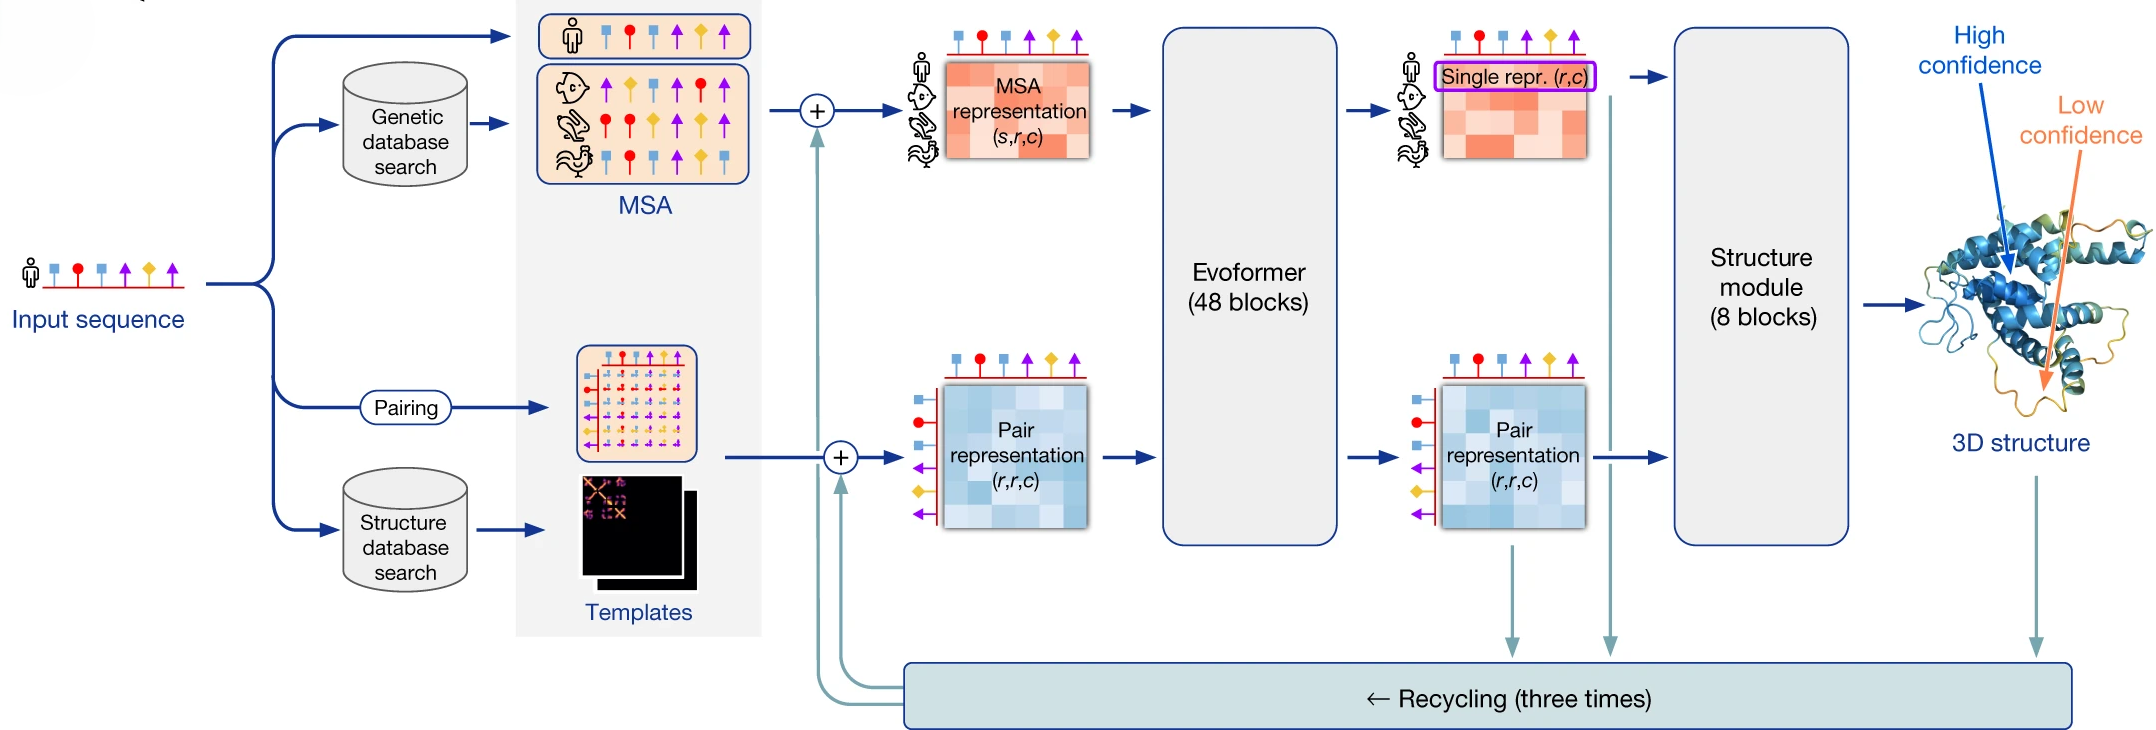
\includegraphics[width=1\linewidth]{figures/alphafold_pipeline.png}
    \caption{Schema semplificato della rete neurale di AlphaFold. Adattato e modificato dall'opera originale di Jumper et al. (2021), disponibile in Open Access sotto licenza Creative Commons Attribution 4.0 International (\url{http://creativecommons.org/licenses/by/4.0/}).}
    \label{fig:alphafold}
\end{figure}






\chapter{DTI e DTA: Predizione delle interazioni Farmaco-Bersaglio}

\section{Il problema computazionale}

Una delle fasi più complesse della pipeline è la corretta predizione delle 
interazioni biochimiche tra il target (precedentemente identificato nella 
\textit{target prediction}) e i possibili farmaci.
Per introdurre modelli matematici e algoritmi di ML in questo step del 
processo è necessario ricondurre la ricerca a un problema computazionale 
ben definito, ovvero prevedere se, e con quale intensità, una determinata 
molecola interagirà con un target specifico.

Il nucleo di questo problema computazionale risiede nella capacità di 
modellare correttamente la \textbf{funzione di interazione} (o funzione 
di \textbf{scoring}).
\begin{equation}
    f(d,t) \xrightarrow{} y
\end{equation}
L'algoritmo ha il compito di filtrare lo spazio chimico come segue: 
data una proteina $t$ (\textit{target}), il modello esplora un dataset 
massivo di sequenze molecolari $\{d_1,d_2,...,d_n\}$ per identificare 
quelle che massimizzano la \textbf{funzione di scoring}.
Questi valori calcolati permettono di creare un \textit{ranking} dei 
potenziali composti candidati e delle interazioni più potenzialmente 
efficaci.
Questo processo è il passaggio cruciale della ricerca farmacologica 
moderna da problema sperimentale biochimico a problema di 
\textbf{ottimizzazione} e ricerca in uno \textbf{spazio latente} a 
dimensionalità alta.

La funzione può determinare, in base alla sua tipologia di output, due 
approcci principali:
\begin{itemize}
    \item \textbf{Classificazione Binaria} \{0,1\}, se il modello 
    fornisce un output booleano, che indica la assenza/presenza di 
    interazione con il target \cite{mondalAIdrivenDrugTarget2026a}.
    \item \textbf{Regressione}, se il modello ritorna un valore continuo 
    che quantifica la forza di legame, ovvero la 
    \textbf{Drug-Target Affinity (DTA)}.
\end{itemize}

\subsection{DTI: classificazione binaria}

\subsection{DTA: regressione del livello di affinità}

L'obiettivo principale della \textit{drug-target affinity} è la stima 
dell'energia libera di legame (ovvero l'affinità di legame) prevista tra 
farmaco e proteina-bersaglio \cite{mondalAIdrivenDrugTarget2026a}.
Questa stima include la previsione di parametri biologici come la 
\textbf{costante di dissociazione} ($K_d$), la \textbf{costante di 
inibizione} ($K_i$) o la \textbf{concentrazione inibente} ($IC_{50}$). 
Una volta calcolati, questi valori vengono convertiti in scala logaritmica 
per stabilizzare la convergenza durante la fase di \textit{training} dei 
modelli di Deep Learning \cite{kumarPredictingDrugtargetInteractions2026a}.

\subsection{Matrice di interazione e DTI Network}
Sia $D$ lo spazio chimico dei farmaci, e $T$ lo spazio biologico dei 
target, l'insieme delle relazioni tra i due può essere formalizzato 
attraverso una \textbf{matrice di interazione} farmaco-bersaglio 
(DTI matrix) \cite{mondalAIdrivenDrugTarget2026a}, in cui le righe 
rappresentano i ligandi, mentre le colonne rappresentano i bersagli 
biologici. 
Di conseguenza, ogni cella $M_{i,j}$ contiene il valore dell'interazione 
tra il farmaco $i$-esimo e il target $j$-esimo (in formato binario per la 
DTI e come valore continuo nella DTA).

Questo tipo di rappresentazione presenta tuttavia una problematica 
strutturale: le matrici di interazione sono infatti estremamente 
\textbf{sparse}, a causa del fatto che la maggior parte delle coppie 
$d$-$t$ non sono mai state testate sperimentalmente e non si hanno quindi 
informazioni a riguardo. 
Per superare tale limite, si ricorre a tecniche di 
\textit{Matrix Factorization} avanzate, come la \textit{Neighbourhood 
Regularized Logistic Matrix Factorization (NRLMF)}, che decompongono la 
matrice in componenti latenti per identificare pattern nascosti e 
prevedere interazioni sconosciute \cite{mondalAIdrivenDrugTarget2026a}.

Tuttavia, questo approccio tratta la matrice come un oggetto isolato e 
non sfrutta le relazioni strutturali tra i composti stessi, come la 
\textbf{similarità} chimica o funzionale tra molecole. 
Per integrare questo tipo di informazioni, le DTI matrix vengono 
reinterpretate come le matrici di adiacenza di una \textbf{DTI Network}.

Si tratta di un \textbf{modello di rete bipartita eterogenea}, in cui i 
nodi di una partizione (composti) sono collegati ai nodi dell'altra 
(target) tramite archi che rappresentano le interazioni note tra i due.
Questa riformulazione supera la staticità della matrice ``piatta'' e 
permette di modellare le relazioni intra-partizione, oltre a quelle 
farmaco-target, arricchendo ulteriormente il quadro informativo per la 
predizione \cite{mondalAIdrivenDrugTarget2026a}.

Modelli di ML supervisionato come il \textit{Bipartite Local Model} (BLM) 
sfruttano questa struttura per costruire dei classificatori \textit{locali} 
specifici per ogni nodo della rete.
A differenza di modelli globali che analizzano la rete nella sua interezza, 
il BLM addestra un classificatore separato per ogni farmaco e ogni target, 
rifacendosi alle interazioni nel \textit{neighbourhood} del nodo come 
segnale supervisionato. Questa strategia permette di catturare pattern 
specifici dei protagonisti dell'interazione, che i modelli globali 
generalizzerebbero eccessivamente.


\section{Metodologie di Predizione}
L'obiettivo è la costruzione di un modello che, in seguito ad un 
addestramento, sia in grado di fare generalizzazioni su coppie 
farmaco-target mai osservate prima, stimando correttamente la probabilità 
di interazione e la sua intensità.

Queste metodologie si differenziano in base al tipo di informazione su 
cui si basano:
\begin{itemize}
    \item I metodi \textbf{ligand-based}, tra cui rientrano i modelli 
    \textbf{QSAR (\textit{Quantitative Structure-Activity Relationship})}, 
    che associano le proprietà strutturali di un determinato composto con 
    la sua attività biologica.
    Storicamente implementati tramite modelli lineari, i modelli QSAR si 
    sono nel tempo evoluti verso modelli di ML e DL di complessità ed 
    efficienza maggiore, rimanendo comunque di natura \textit{ligand-based}.
    Anche la \textbf{modellazione farmacoforica} fa parte di questa 
    categoria, e serve ad identificare le caratteristiche strutturali 
    minime di un composto per ottenere l'interazione desiderata con il 
    bersaglio, stringendo il cerchio di possibili candidati (risulta 
    particolarmente utile nei casi in cui la struttura 3D della proteina 
    non è ricavabile \cite{mondalAIdrivenDrugTarget2026a}).
    \item I metodi \textbf{structure-based} che, al contrario dei 
    precedenti, richiedono la conoscenza della struttura 3D della proteina 
    target, al fine di simulare l'interazione chimica. Il rappresentante 
    principale di questa categoria è il \textbf{docking molecolare}, 
    che verrà trattato nella sezione successiva (\cref{subsec:docking}).
    \item I metodi \textbf{network-based}, comprendono la DTI network e 
    il modello BLM, già citati in precedenza. Questi rappresentano i 
    farmaci e i target attraverso i nodi di un grafo e sfruttano la 
    topologia della rete per analizzare nuove connessioni/interazioni.
    \item I metodi basati su \textbf{Machine Learning} e \textbf{Deep 
    Learning}, infine, rappresentano lo stato dell'arte.
    I modelli di ML classico apprendono pattern complessi a partire da 
    descrittori progettati manualmente, mentre le architetture di DL 
    estraggono automaticamente le informazioni facendo affidamento solo 
    al dataset di input, senza richiedere \textit{feature engineering}.
    Entrambi verranno trattati in dettaglio più avanti.
\end{itemize}

\subsection{Metodi ligand-based e structure-based}
\subsubsection{QSAR e modelli farmacoforici}

\subsubsection{Docking molecolare}
\label{subsec:docking}

\subsection{Machine Learning Classico}

Le metodologie computazionali per la predizione di interazioni 
farmaco-target hanno seguito un processo evolutivo motivato dalle 
limitazioni riportate dalle generazioni precedenti.
I primi approcci si basavano su descrittori delle proprietà molecolari 
dei composti progettati manualmente e basati unicamente sulle competenze 
e conoscenze scientifiche degli esperti di laboratorio.

\subsubsection{Modelli lineari}

I modelli di ML tradizionale si basano spesso sulla \textit{feature 
engineering} manuale, eseguita prima dell'addestramento del modello da 
ricercatori incaricati di selezionare le caratteristiche descrittive delle 
molecole, ovvero le loro proprietà fisico-chimiche.
Tra questi approcci si distinguono i \textbf{Modelli Lineari} 
\cite{odugbemiArtificialIntelligenceAntidiabetic2024}:
\begin{itemize}
    \item \textbf{MLR (Multiple Linear Regression)}
    \item La regressione dei \textbf{minimi quadrati parziali (PLS)}
    \item La \textbf{Regressione Lineare Bayesiana (RLB)}
\end{itemize}
Questi rappresentano tecniche statistiche in grado di generare una 
funzione lineare che descrive il legame tra i descrittori molecolari 
(le variabili $x$, dette ``indipendenti'') e l'esito della predizione, 
ovvero l'affinità di legame (variabili $y$, ``dipendenti'') 
\cite{odugbemiArtificialIntelligenceAntidiabetic2024}. 
In questo modo, il modello è capace di calcolare come i cambiamenti nelle 
proprietà dei composti influenzino l'attività biologica di essi. Diventa 
quindi possibile prevedere il comportamento di nuovi composti da analizzare, 
semplicemente ``consultando'' la linea di regressione e inserendo i nuovi 
parametri nella funzione.

Il limite di questi modelli, tuttavia, risiede proprio nella loro 
possibilità di catturare unicamente relazioni lineari, escludendo quindi 
pattern di interazione più complessi.

\subsubsection{Alberi decisionali e Random Forest}

Per superare questo ostacolo di complessità subentrano metodi più avanzati, 
come \textbf{Random Forest} e gli \textbf{alberi di decisione} (\textbf{DT}), 
che sono in grado di ricavare dai dati relazioni complesse, rappresentabili 
da funzioni non-lineari.

I \textbf{DT} sono una struttura dati ad albero in cui i dati vengono 
ricorsivamente partizionati in sottoinsiemi in base a caratteristiche 
specifiche come, in questo caso, particolari proprietà molecolari. 
In questo modo i rami della struttura rappresentano i possibili esiti del 
problema di classificazione/regressione (in base al tipo di task che viene 
affrontato, DTI o DTA).
Una volta ``riempito'', il DT può essere usato come modello predittivo, 
in grado di classificare nuovi composti in base al loro percorso guidato 
dalla radice fino alle foglie dell'albero 
\cite{odugbemiArtificialIntelligenceAntidiabetic2024}.
Queste tecniche sono efficaci e facili da interpretare, ma soffrono di 
\textbf{overfitting}: 
indeed, questi modelli tendono a ``memorizzare'' le caratteristiche dei 
dati del \textit{training set}, senza realmente apprendere dei pattern 
per generalizzare il comportamento dei vari input. In questo modo, le 
prestazioni risultano eccellenti durante la fase di training ma abbastanza 
scarse durante la fase di test o l'identificazione di nuovi dati.

La \textbf{Random Forest (RF)} è una tecnica di \textit{ensemble learning} 
progettata per ridurre il fenomeno di overfitting. È composta da più DT 
combinati e addestrati su sottoinsiemi differenti del dataset generale. 
La decisione finale avviene tramite voto di maggioranza, nel caso della 
DTI, o tramite media, nel caso della DTA.

\subsubsection{Support Vector Machines}

Oltre agli algoritmi \textit{tree-based}, sono utilizzate anche tecniche 
come \textbf{Support Vector Machines (SVM)}. Queste affrontano la 
classificazione DTI cercando, all'interno dello spazio dei descrittori, 
l'\textbf{iperpiano di separazione} con margine massimo tra coppie in 
interazione e non interagenti.
L'iperpiano ottimale è quello che massimizza la distanza tra i punti più 
vicini di ciascuna delle due classi, infatti più il margine è ampio e 
migliore sarà la capacità del modello di fare previsioni su coppie mai 
osservate. 
Questi punti ``di confine'' vengono chiamati \textbf{vettori di supporto} 
e garantiscono la stabilità del sistema 
\cite{montesinoslopezSupportVectorMachines2022}. 

Per gestire la non-linearità delle proprietà biologiche, SVM ricorre al 
\textbf{kernel trick}, che ``solleva'' i dati di una dimensione, 
garantendo sempre la separazione lineare. 
Il kernel non necessita delle coordinate dei punti nello spazio, ma 
ricava direttamente il loro \textbf{prodotto scalare} calcolandolo in uno 
spazio a dimensionalità superiore 
\cite{montesinoslopezSupportVectorMachines2022}. 

Il limite strutturale comune a tutti gli approcci di ML tradizionale è 
la dipendenza della predizione dalla qualità dei descrittori selezionati 
\cite{ahmadMachineLearningDrugtarget2026}.
L'inadeguatezza delle proprietà molecolari in esame può compromettere il 
lavoro del modello indipendentemente dalla sua potenza di calcolo o dalla 
sua efficienza.
Questo vincolo è proprio la motivazione del passaggio verso le architetture 
di \textbf{Deep Learning}, in grado di apprendere in modo autonomo le 
informazioni dai dataset.

\subsection{Deep Learning}
Il subentro del \textbf{Deep Learning} ha affrontato i problemi di DTI e 
DTA come un \textbf{task di apprendimento supervisionato}: il modello 
apprende la funzione
\begin{equation}
    f(d,t) \xrightarrow{} y
\end{equation}
in grado di generalizzare su coppie drug-target non osservate, 
riconoscendo pattern chimici e biologici di alta complessità.
Invece di ricevere parametri calcolati manualmente, questi modelli ricavano 
le caratteristiche più informative direttamente dai dati ``grezzi'', siano 
questi stringhe SMILES, sequenze amminoacidiche o grafi molecolari 
\cite{wangUnifiedSurveyDrugtarget2026a}.

\subsubsection{Modelli sequence-based (CNN, RNN/LSTM)}

I modelli \textit{sequence-based} affrontano il problema DTI trattando 
direttamente le stringhe SMILES o i fingerprint del farmaco e le sequenze 
delle proteine come dati testuali unidimensionali, senza richiedere input 
formalizzati ``su misura'' \cite{tangTCDTAPredictingDrugTarget2024a}.

\paragraph{CNN:}

Le \textbf{CNN} o \textbf{Reti Neurali Convoluzionali} rappresentano una 
delle prime architetture DL applicate con successo a questo tipo di input 
biologico.
Nascono principalmente per processare dati in formato a griglia come i 
pixel nelle immagini, ma possono essere adottate in ambito di predizione 
DTI e DTA per lavorare su task di QSAR, tramite \textbf{convoluzione 
unidimensionale} \cite{odugbemiArtificialIntelligenceAntidiabetic2024}.
Il processo si divide in tre fasi principali che seguono i diversi strati 
della rete:
\begin{itemize}
    \item \textbf{Layers Convoluzionali}, che scansionano le sequenze dei 
    composti e ricercano al loro interno dei pattern strutturali locali, 
    detti \textit{\textbf{motif}}.
    Il risultato del passaggio attraverso questi strati è la composizione 
    di una matrice \textbf{feature map}, che indica le feature estratte e 
    il grado di certezza nella loro rilevazione.
    \item \textbf{Layers di Pooling}, che riducono la dimensionalità delle 
    feature map ottenute, riassumendo solo le informazioni più importanti 
    e utili per la previsione di nuovi composti. Questo step, oltre a 
    rendere il modello più leggero, è fondamentale per la riduzione del 
    \textit{noise}, ovvero informazioni superflue che potrebbero 
    compromettere il risultato del procedimento con piccole variazioni di 
    misurazione e impurità nei dati.
    \item \textbf{Layers Fully Connected}, infine, sono strati densi che 
    combinano tra loro le caratteristiche apprese dalle mappature nei 
    livelli precedenti, per generare una previsione finale.
\end{itemize}

Questo tipo di reti neurali sono facilmente scalabili e molto efficienti 
ma, facendo uso di informazioni 1D, fanno anch'esse fatica ad incorporare 
strutture tridimensionali più complesse e a catturare le dipendenze 
biochimiche tra elementi \cite{houDGCADTADeepGraph2025}.

\paragraph{RNN:}

Le \textbf{RNN (Recurrent Neural Networks)} sono un'altra architettura 
di Deep Learning progettata per l'elaborazione di dati sequenziali. 
A differenza delle CNN, però, queste reti non sono in grado di modellare 
in modo corretto e affidabile le dipendenze tra atomi tra loro distanti 
\cite{wangUnifiedSurveyDrugtarget2026a}.

Operano mantenendo un \textbf{layer nascosto}, che si evolve con 
l'elaborazione della sequenza di input. 
Nel contesto della predizione di interazioni con il target farmacologico, 
le RNN, come le CNN, analizzano efficacemente le stringhe SMILES dei 
composti per apprendere i \textbf{motifs} strutturali e i pattern nelle 
relazioni che determinano l'affinità di legame.

\subsubsection{Modelli graph-based (GNN)}

I modelli \textit{sequence-based}, anche se risultano più semplici nella 
formattazione degli input e più facilmente scalabili, faticano a prendere 
conoscenza del contesto tridimensionale del sito di legame 
\cite{wangUnifiedSurveyDrugtarget2026a}. Questa perdita di informazioni 
può essere superata grazie alla rappresentazione a grafo tipica dei modelli 
trattati in questa sezione.

Come accennato brevemente nel capitolo precedente, questo tipo di rappresentazione 
permette l'elaborazione dei contesti da parte delle \textbf{GNN (Graph 
Neural Networks)}, che operano simulando la topologia e le relazioni 
spaziali reali dei composti chimici (legami tra atomi \textit{intra} e 
\textit{inter} composto) propagando informazioni tra i nodi tramite il 
meccanismo di \textit{message passing}. Questo processo avviene 
in due passaggi iterativi \cite{wangGraphNeuralNetworks2023}:
\begin{itemize}
    \item \textbf{Computazione e Aggregazione:} Il modello calcola un 
    messaggio elaborando le caratteristiche del nodo centrale, con quelle 
    dei nodi e degli archi ad esso adiacenti.
    \item \textbf{Aggiornamento:} Lo stato del nodo viene aggiornato 
    integrando il nuovo messaggio con la sua informazione precedente.
\end{itemize}

Queste informazioni elaborate vengono poi lette tramite l'operazione di 
\textbf{Readout}. Attraverso un meccanismo simile al pooling, le 
caratteristiche di tutti i nodi vengono aggregate e aggiornate in un 
unico vettore di caratteristiche globali, in grado di rappresentare lo 
stato dell'intera molecola \cite{wangGraphNeuralNetworks2023}.

In generale, nel contesto di drug discovery le GNN stanno rivoluzionando 
il concetto di tradizionale \textbf{Computer-Aided Drug Design} (CADD), 
trasformando il processo in una ricerca automatizzata.
Queste architetture consentono di esplorare lo spazio chimico per generare 
e ottimizzare (come nella \textit{Lead Optimization}) nuove entità 
molecolari, apportando migliorie nelle proprietà desiderate, come 
bioattività, stabilità e sintetizzabilità. 
Queste permettono anche uno studio precoce di proprietà ADMET e della tossicità, 
portando a una riduzione drastica di fallimenti nei test clinici 
\cite{wangGraphNeuralNetworks2025}.

Nel contesto del problema computazionale DTI/DTA, le GNN risultano fondamentali nello screening virtuale per prevedere con efficienza le affinità di legame tra farmaci e target attraverso l'implementazione di architetture a doppia branca (\textit{dual-branch}). In questo paradigma, il problema predittivo viene convertito in un compito di fusione di informazioni estratte in parallelo da due grafi distinti:

\begin{itemize}
    \item \textbf{Branca del Farmaco ($d$):} La piccola molecola viene convertita in un grafo molecolare in cui gli atomi rappresentano i nodi (caratterizzati da proprietà chimiche come numero atomico, valenza, ecc...) e i legami chimici costituiscono gli archi. Algoritmi come le \textit{Graph Convolutional Networks} (GCN) scansionano questa struttura per estrarre pattern locali e stereochimici stabili.
    \item \textbf{Branca del Target ($t$):} La proteina viene modellata come un grafo di contatto dei residui. In questa struttura, i nodi rappresentano i singoli amminoacidi, mentre gli archi vengono tracciati tra nodi la cui distanza euclidea nello spazio 3D è inferiore a una determinata soglia, preservando la topologia del sito di legame \cite{ahmadMachineLearningDrugtarget2026}.
\end{itemize}

Una volta che i messaggi sono stati propagati all'interno delle rispettive strutture, le operazioni di \textit{readout} generano \textbf{due vettori di feature ad alta dimensionalità}. Questi vettori vengono successivamente combinati all'interno di un modulo di interazione, spesso arricchito da meccanismi di attenzione (\textit{Graph Attention Networks} - GAT) per pesare l'importanza relativa dei vari atomi e residui nel complesso farmaco-bersaglio \cite{ozsariDTAGNNToolkitConstructing2026}. Il vettore risultante viene infine processato da strati \textit{Fully Connected} per mappare l'interazione nell'output finale $y$, traducendosi in una classificazione booleana per i task di DTI o in un valore continuo di affinità ($K_d$, $K_i$, $IC_{50}$) per i task di DTA.

\subsubsection{Modelli attention-based e Transformer}

Le architetture basate sul meccanismo di \textbf{attenzione} e sui 
\textbf{Transformer} rappresentano l'attuale stato dell'arte nella 
predizione di DTI e DTA. Il loro punto di forza principale risiede nella 
capacità di catturare \textbf{dipendenze a lungo raggio} all'interno delle 
sequenze molecolari e proteiche \cite{ahmadMachineLearningDrugtarget2026} \cite{mondalAIdrivenDrugTarget2026a}, superando il limite strutturale delle CNN 
e delle RNN, che tendono a perdere il contesto globale quando le sequenze 
diventano molto lunghe.

\paragraph{Il meccanismo di attenzione}

L'\textit{attention} si basa sulla premessa che non tutte le parti di 
una sequenza sono ugualmente rilevanti per una previsione. 
Si rende quindi necessario \textbf{pesare selettivamente} le sottosequenze più 
informative, ad esempio, applicato alle interazioni farmaco-bersaglio, i residui amminoacidici del sito di legame, ignorando le regioni che non contribuiscono all'interazione.
% figura? heatmap


\paragraph{Architetture Transformer per DTI e DTA}

I \textbf{Transformer} estendono il meccanismo di attention trattando le stringhe SMILES e le sequenze 
amminoacidiche (FASTA) come se fossero un linguaggio naturale da 
interpretare. 
A differenza delle RNN, che elaborano i token uno alla 
volta in modo sequenziale, i Transformer processano l'intera sequenza 
simultaneamente, rendendo il training più efficiente e la cattura del 
contesto globale più affidabile \cite{wangUnifiedSurveyDrugtarget2026a}.
% figura di architettura generale di un Transformer encoder

Tra i modelli più rappresentativi si distinguono:
\begin{itemize}
    \item \textbf{MolTrans} e \textbf{MT-DTI}, che applicano encoder 
    Transformer sia al farmaco che alla proteina per apprendere 
    rappresentazioni consapevoli del contesto. Questi modelli mostrano 
    ottime prestazioni anche in scenari \textit{cold-start}, ovvero in 
    presenza di coppie farmaco-target nuove mai osservate durante il training \cite{mondalAIdrivenDrugTarget2026a}.
    \item \textbf{TC-DTA}, un modello ibrido che adotta un encoder 
    Transformer per la sequenza proteica e una CNN per la rappresentazione 
    del farmaco, ottimizzando l'estrazione di informazioni semantiche 
    dagli amminoacidi pur mantenendo l'efficienza computazionale della rete
    convoluzione per il lato molecolare \cite{tangTCDTAPredictingDrugTarget2024a}.
    \item \textbf{FusionDTI}, che integra token strutturali proteici e 
    stringhe SELFIES tramite Transformer, con l'obiettivo di ottenere 
    predizioni a grana fine sul sito di legame specifico.
\end{itemize}

\paragraph{Graph Transformer}
Un'ulteriore evoluzione consiste nell'applicare la logica dei Transformer 
direttamente alle strutture a grafo delle molecole, dando origine ai 
cosiddetti \textbf{Graph Transformer}. Questi modelli incorporano nei 
meccanismi di \textit{attention} informazioni strutturali specifiche del grafo, 
come la \textbf{centralità dei nodi} e le \textbf{distanze spaziali} tra 
atomi, che le GNN standard non sfruttano in modo esplicito.
Il modello \textbf{GraphormerDTI} rappresenta un esempio di questa 
categoria applicata al problema DTI, dimostrando miglioramenti rispetto 
alle GNN classiche grazie all'integrazione di queste feature informative strutturali 
nell'attenzione \cite{kumarPredictingDrugtargetInteractions2026a}.

\paragraph{Modelli linguistici pre-addestrati (PLM)}
I Transformer costituiscono la spina dorsale dei cosiddetti 
\textbf{Foundation Models}, ovvero modelli pre-addestrati su database 
massivi in modalità auto-supervisionata e successivamente adattati a 
compiti specifici tramite \textit{fine-tuning}. Questo paradigma 
\textit{pre-train / fine-tune} permette di sfruttare la conoscenza 
biochimica e chimica generale acquisita su larga scala verso i task di DTI e DTA 
con dataset di dimensioni più ridotte \cite{wangUnifiedSurveyDrugtarget2026a}.

\paragraph{Vantaggi e limiti}
Uno dei punti di forza più rilevanti di questi modelli in ambito 
farmacologico e/o medico è la loro \textbf{interpretabilità}: i pesi di attenzione 
possono essere visualizzati attraverso delle \textbf{mappe di attenzione}, che indicano 
quali atomi o residui hanno guidato maggiormente la predizione \cite{kumarPredictingDrugtargetInteractions2026a}. Questo 
strumento offre ai ricercatori la possibilità di \textbf{validare 
biologicamente} il risultato computazionale, verificando se le regioni 
evidenziate corrispondono a siti di legame noti.
% figura saliency map ?

Il principale limite rimane la \textbf{complessità computazionale}: 
l'\textit{attention} ha complessità quadratica rispetto alla lunghezza della 
sequenza, il che rende il training particolarmente oneroso in termini di 
tempo e memoria quando si lavora con sequenze proteiche molto lunghe \cite{mondalAIdrivenDrugTarget2026a}

%\subsubsection{Modelli ibridi}
\chapter{ADMET}
La valutazione delle proprietà \textbf{ADMET} (Assorbimento, Distribuzione, Metabolismo, Escrezione e Tossicità) è considerata un passaggio critico all'interno della pipeline di svilluppo farmacologico, al fine di ridurre "a monte" i tassi di fallimento nelle fasi cliniche. Infatti, la scorretta valutazione di queste proprietà rappresenta un incremento nel rischio di logoramento dei farmaci candidati.

\section{Il framework ADMET}
L'impiego del Machine Learning in questo campo rappresenta un'importante svolta metodologica rispetto ai test empirici tradizionali \cite{Yang2021}, poiché permette di processare grandi volumi di dati molecolari per prevederne il comportamento farmacocinetico con costi e tempi drasticamente ridotti, allargando il primo "collo di bottiglia" del processo di ricerca.

In questo nuovo contesto, il framework ADMET non viene più interpretato come una serie di test isolati, ma come un sistema integrato di vincoli biochimici che si influenzano a vicenda e che determinano la sicurezza di una molecola. 

\section{La tossicità molecolare}
TO-DO

\section{Evoluzione verso il Machine Learning per la predizione ADMET} %da li2026
Storicamente, i primi tentatici di razionalizzare le proprietà e l'attività biologica delle molecole si basava su metodi come \textit{quantitative structure-activity relationship} (QSAR) e \textit{structure-activity relationship} (SAR).
Tuttavia questi metodi presentavano un limite fondamentale: la necessità di una selezione manuale e di un'accurata rappresentazione delle \textit{feature} chimiche. %Approfondisci
Con l'avvento del ML classico, tuttavia, l'attenzione si è spostata verso l'uso di rappresentazioni come i \textit{chemical fingerprints}, che vengono presi come input da algoritmi come \textbf{Random Forest}, \textbf{Support Vector Machines}, \textbf{k-Nearest Neighbors} e \textbf{XGBoost}. 
Questi ultimi hanno permesso di apprendere classificazioni complesse, trattando la molecola come un vettore binario che indica presenza/assenza di frammenti chimici, e raggiungendo risultati in modo veloce e con processi parzialmente interpretabili.
Tuttavia, questi algoritmi ignorano la struttura tridimensionale e la connettività delle molecole, e le leggono invece come una sequenza di caratteristiche booleane, rendendo le interazioni tra frammenti vicini nello spazio ma lontani nella stringa di difficile predizione.

Per una predizione più accurata di queste interazioni più complesse, \textbf{Li et al. (2026)} propongono un modello chiamato \textbf{CMA}, ovvero "Cross-Aligned Multimodal Attention". 
L'idea centrale è proprio quella di rappresentare la molecola come in un \textbf{attention cross-modale}, ovvero tramite tre le matrici Query (Q), Key (K) e Value (V) del meccanismo di attentio dei Transformer. Ogni matriche viene mappata a partire da una rappresentazione diversa, e solo una di queste fa riferimento ai \textit{fingerprints}:
\begin{itemize}
    \item Query utilizza \textbf{GROVER}, un algoritmo che decodifica informazioni sulla struttura delle molecole in un grafo in cui ogni nodo rappresenta un atomo e i legami chimici sono astratti come archi. GROVER è un \textbf{GNN} (Graph Neural Networks) preaddestrato su 10 milioni di molecole e permette la la rappresentazione più ricca strutturalmente. Contruibuisce a circa il 36\% della contibuzione media finale.
    \item Value viene processata da \textbf{ResNet-50}, una CNN in grado di estrarre immagini molecolari bidimensionali e catturare così la forma, la simmetria e l'arrangiamento degli atomi dei soggetti candidati. La rete viene preaddestrata su 10 milioni di molecole. Contruibuisce a circa il 22\% della contibuzione media finale.
    \item Key, infine, fa uso di \textbf{fingerprint MACCS}, composta da 166 bit che codifica l'occorrenza di gruppi chimici specifici. Contruibuisce a circa il 42\% della contibuzione media finale.
\end{itemize}
La funzione di punteggio di Attention è definita come segue:
$$\text{Attention}(Q, K, V) = \text{softmax}\left(\frac{QK^T}{\sqrt{d_k}}\right)V$$
La modalità Query "interroga" la modalità Key per determinare quali elementi siano più rilevanti all'interno del contesto corrente. Il risultato è infine un media pesata dalla modalità Value. Tradotto nell'ambito molecolare, la rappresentazione a grafo può interrogare le \textit{fingerprint} per comprendere al meglio quali siano le caratteristiche strutturali locali più coerenti con la topologia generale, mentre il risultato finale viene modulato dalle immagini estratte da ResNet. 
%TO_DO interpretabilità e gradcam
\cite{li2026}

\section{Multimodalità e meccanismi di Attention}
%\section{Modelli predittivi/GNN per la previsione della sicurezza}
\chapter{Applicazioni di successo}
Osserviamo ora alcuni modelli di Intelligenza 
Artificiale che si sono dimostrati in grado di produrre risultati concreti e validati 
clinicamente. 
I tre casi documentati di seguito illustrano come i 
metodi trattati in questo elaborato abbiano già cambiato 
la pratica della \textit{drug discovery}.

\section{Baricitinib per COVID-19}
Nel 2020, il team di BenevolentAI ha pubblicato 
su \textit{The Lancet} un'analisi che illustra come una rappresentazione a  
\textbf{knowledge graph} avanzato, costruito come un archivio strutturato di 
informazioni biologiche e mediche estratte tramite ML,
abbia permesso di identificare in pochi giorni il 
\textbf{baricitinib} come potenziale trattamento per 
l'infezione da SARS-CoV-2 
\cite{richardsonBaricitinibPotentialTreatment2020}.

Il baricitinib è un inibitore delle chinasi Janus (JAK), 
già conosciuto e approvato per il trattamento dell'artrite reumatoide. 
Gli algoritmi di predizione DTI di BenevolentAI hanno 
identificato la sua capacità di inibire la proteina 
\textbf{AAK1}, un regolatore dell'endocitosi (il meccanismo attraverso cui il virus entra nelle cellule 
polmonari). Questo ha suggerito un duplice meccanismo 
d'azione: 
\begin{itemize}
    \item La riduzione dell'ingresso virale all'interno dei tessuti polmonari.
    \item La modulazione della risposta infiammatoria nel caso di avvenuta contaminazione.
\end{itemize}
Il farmaco ha successivamente ricevuto l'autorizzazione d'uso 
emergenziale, dimostrando un beneficio significativo 
sulla mortalità nei pazienti con COVID-19 grave.

Questo caso è emblematico del \textbf{drug repurposing 
guidato da ML}, ovvero la capacità di identificare nuovi 
target biologici per farmaci già approvati, 
riducendo drasticamente i tempi di validazione 
clinica.
Si tratta una delle applicazioni più immediate 
e ad efficaci dei metodi di predizione DTI 
discussi in questo elaborato.

\section{Halicin: un antibiotico scoperto dal Deep 
Learning}
Nel 2020, un gruppo di ricercatori del MIT ha pubblicato 
su \textit{Cell} la scoperta di \textbf{Halicin}, il 
primo antibiotico ad ampio spettro identificato tramite 
un approccio di deep learning 
\cite{stokesDeepLearningApproach2020}.

Il modello adottato è \textit{Chemprop}, un'architettura \textbf{D-MPNN} (\textit{Directed Message Passing Neural Network}). Si tratta di una variante delle GNN (descritte nei capitoli precedenti) con lo scopo di prevedere l'attività antibatterica a partire dalla struttura chimica del composto, espressa sotto forma di grafo.

Il modello traduce la rappresentazione in un vettore tramite \textit{message passing}, per costruire una comprensione della chimica locale della molecola.

Il vantaggio rispetto ai metodi tradizionali che fanno uso di fingerprint Morgan o descrittori RDKit (che nel paper vengono usati come \textit{baseline}), è che il \textit{message passing} permette l'apprendimento automatico in funzione della proprietà da predire, senza aver la necessità di introdurre definizioni manuali.
Tuttavia, per aumentare le prestazioni della rete neurale, sono stati concatenate alla rappresentazione iniziale, 200 descrittori chimici classici (da RDKit) per bilanciare la difficile propagazione dei messaggi su grafi molecolari molto estesi.

Successivamente è avvenuta la fase di \textit{training}, svolto per il task di classificazione DTI su molecole in grado di inibire la crescita di \textit{E. coli}. Vengono coinvolte nello screening 2.560 molecole e vengono identificate come \textit{hit} 120 composti attivi (5.14\%).
Dopo deduplicazione, il dataset finale è di 2.335 molecole, binarizzate come hit/non-hit.

Il training viene sottoposto a un \textit{fine tuning} attraverso l'\textbf{ottimizzazione Bayesiana dei parametri}, che usa \textit{Bayesian optimization} con 20 iterazioni, esplorando diverse tipologie di iperparametri.

\begin{table}[ht]
    \centering
    \caption{Elenco degli iperparametri del modello.}
    \label{tab:iperparametri}
    \begin{tabular}{lcc}
        \toprule
        \textbf{Hyperparameter} & \textbf{Range} & \textbf{Value} \\
        \midrule
        Number of message-passing steps & [2, 6] & 5 \\
        Neural network hidden size      & [300, 2400] & 1600 \\
        Number of feed-forward layers   & [1, 3] & 1 \\
        Dropout probability             & [0, 0.4] & 0.35 \\
        \bottomrule
    \end{tabular}
\end{table}

Inoltre, il modello finale utilizza un \textit{ensemble} di 20 istanze pesate in modo diverso per aumentare la robustezza della predizione.

La predizione avviene tramite applicazione sulla \textbf{Drug Repurposing Hub}, completa di 6.111 molecole da cui vengono escluse quelle già presenti nel Training-Set.
Vengono individuate le 99 candidate con punteggi più alti, che passano alla fase di testing sperimentalmente. Di queste, 51 si confermano veri positivi.

Un modello Chemprop specifico viene poi addestrato sul dataset \textbf{ClinTox} per prevedere la tossicità delle molecole candidate rimaste.
Ognuna delle entry del dataset è composta da due proprietà binarie, la tossicità rilevata negli studi clinici e lo stato di approvazione della FDA.

Un \textit{ensemble} di 5 modelli seleziona infine \textbf{Halicin} come antibiotico migliore. Si tratta di un inibitore della c-Jun N-terminal kinase originariamente sviluppato per il diabete.

Il risultato informaticamente più rilevante è che 
Halicin ha una struttura chimica radicalmente diversa 
da tutti gli antibiotici convenzionali. Il modello ha quindi dimostrato capacità di \textbf{scaffold hopping},
apprendendo relazioni struttura-attività che sfuggirebbero
all'intuizione umana dei ricercatori e superando il bias
verso strutture chimiche note tipico dei metodi tradizionali.

Testata su modelli murini, 
Halicin ha eliminato infezioni da 
\textit{Clostridioides difficile} e 
\textit{Acinetobacter baumannii} che resistono 
agli antibiotici convenzionali.

Infine, espandendo lo 
screening al database \textbf{ZINC15}, composto da oltre 107 
milioni di molecole, il modello ha identificato in 4 giorni
ulteriori otto composti antibatterici strutturalmente 
distanti dai farmaci noti \cite{stokesDeepLearningApproach2020}.
\section{Rentosertib: il primo farmaco end-to-end 
generato dall'AI}
Il caso più avanzato e recente è quello del 
\textbf{rentosertib} (ISM001-055), sviluppato da 
Insilico Medicine e documentato in uno studio pubblicato su 
\textit{Nature Medicine} nel giugno 2025 
\cite{xuGenerativeAIDiscoveredTNIK2025}.

A differenza dei casi precedenti, i quali applicano ML 
a composti già esistenti, il rentosertib rappresenta 
il primo farmaco in cui sia il \textbf{target biologico} 
che la \textbf{struttura molecolare} del composto sono stati 
identificati o progettati interamente da algoritmi di 
AI generativa.

La piattaforma \textbf{PandaOmics} ha 
identificato \textbf{TNIK} come target critico per la 
fibrosi polmonare idiopatica (IPF), una patologia 
progressiva e attualmente incurabile. La piattaforma 
di chimica generativa ha poi progettato il suo 
inibitore, completando l'intera pipeline dalla target 
identification al candidato preclinico in 
\textbf{soli 18 mesi} (tempi molto ridotti in confronto alle pipeline tradizionali), con meno di 80 molecole 
sintetizzate e testate.

La generazione dell'inibitore specifico di TNIK è avvenuta tramite la piattaforma di chimica generativa \textit{Chemistry42}. Questa ha messo in parallelo 30 modelli generativi che, basandosi su metriche di valutazione e vincoli strutturali condivisi, hanno permesso un'esplorazione dello spazio chimico collaborativa e priva di ridondanze \cite{renSmallmoleculeTNIKInhibitor2025}.

Il sito di legame selezionato come luogo dell'interazione con il bersaglio è risultato il
\textbf{sito di legame dell'ATP di TNIK}.
La generazione è stata vincolata dalle seguenti ipotesi 
\textbf{farmacoforiche} \cite{renSmallmoleculeTNIKInhibitor2025}: 
\begin{enumerate}
    \item Le strutture 
    candidate devono formare un legame idrogeno con 
    l'NH di \textbf{Cys108} nella regione "hinge" (snodo flessibile) della 
    chinasi.
    \item I centri idrofobici devono essere posizionati nello spazio adiacente al gatekeeper \textbf{Met105} (amminoacido che determina l'accessibilità al sito attivo).
\end{enumerate}
Questi vincoli strutturali, gestiti dai moduli 
\textit{Pocket} e \textit{Pharmacophore} della 
piattaforma, guidano la generazione verso strutture 
con le caratteristiche di binding necessarie 
per l'inibizione dell'ATP.

Infine, algoritmi di screening secondari rifiniscono la selezione scartando le strutture chimicamente instabili o troppo complesse da sintetizzare. Questo stringente processo di filtraggio computazionale converte un immenso spazio di generazione in un set ristretto di molecole ad alto potenziale, massimizzando il tasso di successo della sperimentazione in vitro \cite{renSmallmoleculeTNIKInhibitor2025}.
\chapter{Conclusioni}

\section{Sintesi del Lavoro}
Questa tesi ha ripercorso l'evoluzione degli strumenti 
computazionali applicati alla pipeline di sviluppo farmaceutico, 
con un focus sulla predizione delle interazioni farmaco-bersaglio 
e sulla valutazione delle proprietà ADMET. 
Il filo conduttore 
che attraversa tutti i capitoli è il modo in cui la ricerca si è trasformata da un 
processo empirico incerto a un 
problema computazionale di ottimizzazione in spazi ad alta dimensionalità, 
affrontabile attraverso strumenti di apprendimento automatico.

Il capitolo sulla rappresentazione molecolare ha mostrato come 
il primo ostacolo computazionale, ovvero la traduzione di entità biochimiche 
complesse in formati leggibili ed elaborabili da algoritmi, sia stato 
affrontato attraverso rappresentazioni progressivamente più 
espressive:

dalle stringhe SMILES ai fingerprint molecolari, 
fino ai grafi molecolari che preservano la topologia e le caratteristiche
stereochimiche particolari alle singole molecole. 

Il capitolo sulla DTI e DTA ha mostrato come la formalizzazione 
del problema computazionale abbia 
permesso di riformulare la ricerca farmacologica in due task 
distinti di apprendimento supervisionato:

\textbf{classificazione binaria} per la presenza dell'interazione e \textbf{regressione} su valore continuo per 
la stima quantitativa dell'affinità. L'evoluzione dei metodi, 
dai modelli lineari QSAR al docking molecolare fino alle 
architetture di Deep Learning, rispecchia l'avanzamento tecnologico moderno e la crescente
complessità delle relazioni che i modelli sono chiamati a 
catturare.

Il capitolo ADMET ha completato il quadro mostrando come la 
valutazione della sicurezza farmacologica, storicamente 
relegata alle fasi cliniche avanzate, possa essere anticipata 
computazionalmente, riducendo il tasso di logoramento dei 
candidati nelle fasi più costose della pipeline.
\section{Lo Stato dell'Arte e le Sfide Aperte}
Nonostante i progressi documentati, il campo presenta sfide 
algoritmiche e metodologiche ancora aperte che condizionano 
l'affidabilità e la generalizzabilità dei modelli.

Il \textbf{cold-start problem} rimane la sfida critica più 
rilevante. Sebbene molti algoritmi eccellano in scenari "warm", in cui le molecole del Test-Set assomigliano a quelle dell'addestramento, la predizione di interazioni per farmaci o target \textbf{mai 
osservati} durante il \textit{training} richiede modelli con 
capacità di generalizzazione induttiva che le architetture 
attuali possiedono solo parzialmente \cite{wangUnifiedSurveyDrugtarget2026a}.
\begin{figure}
    \centering
    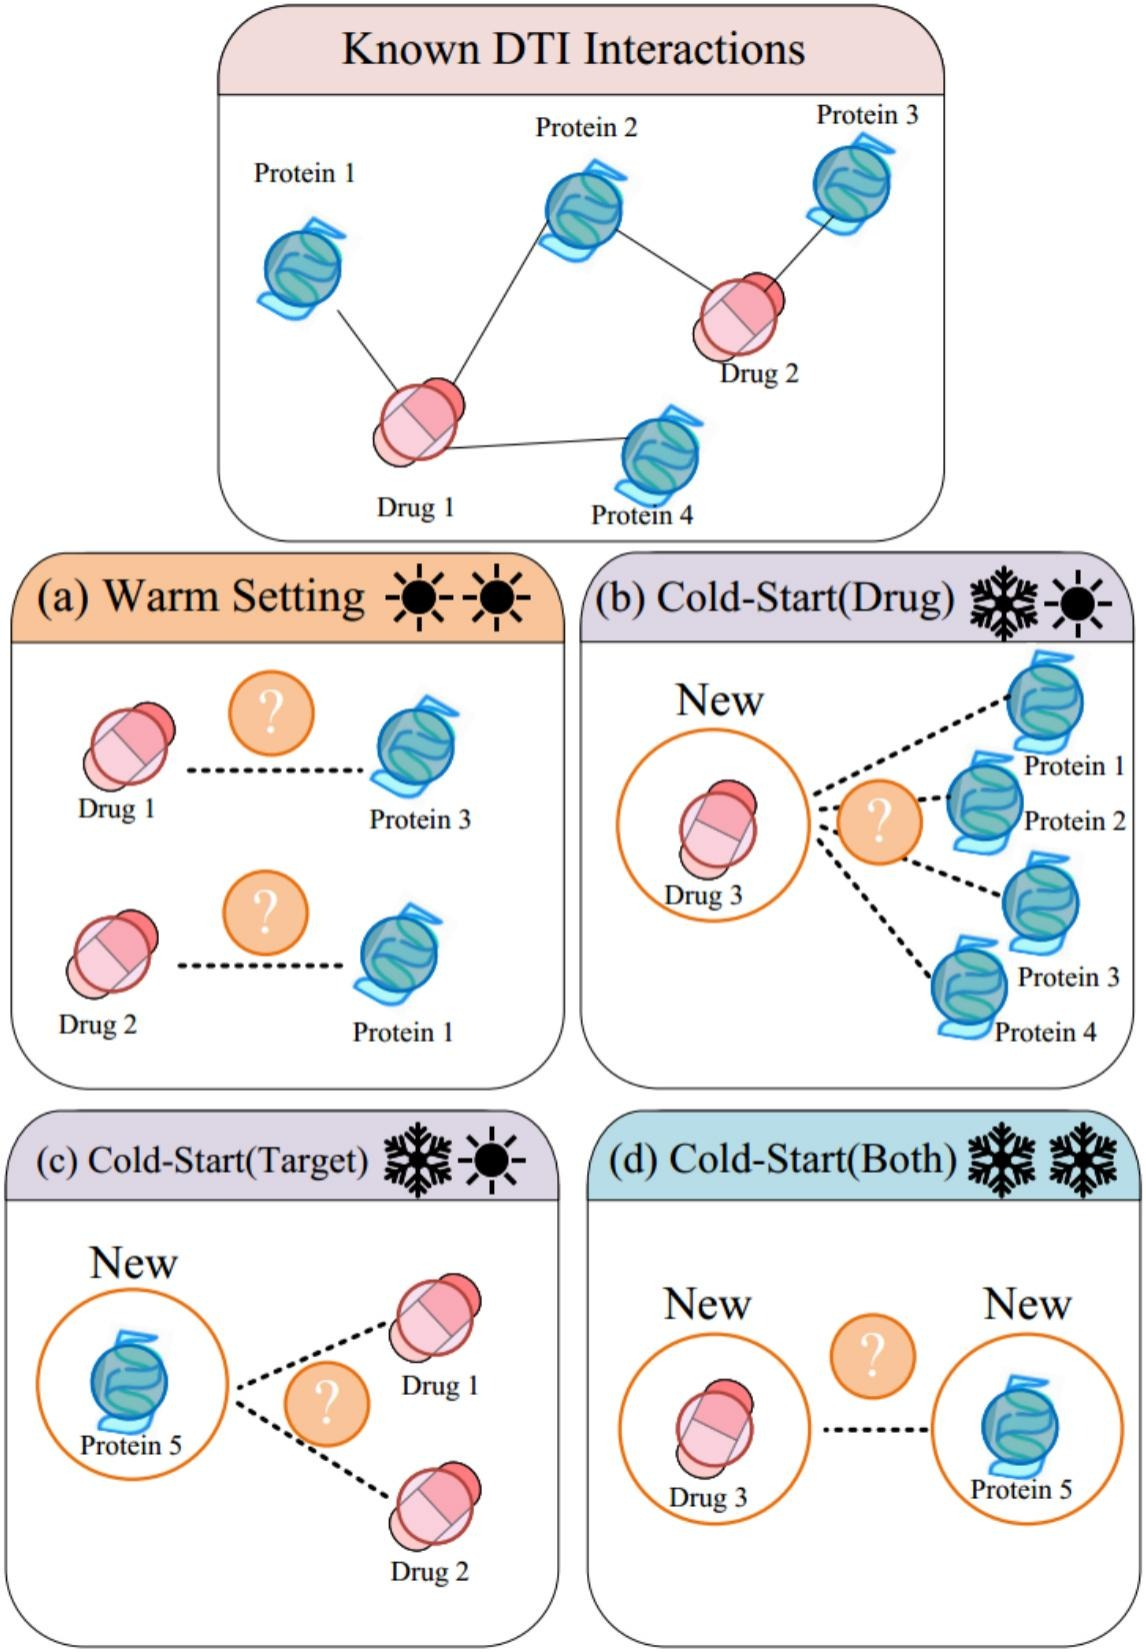
\includegraphics[width=0.5\linewidth]{figures/cold_start.png}
    \caption{(a) Warm-Start: il modello prevede interazioni tra farmaci e target già presenti nel training set. (b) Cold-Start (Drug): predizione per un nuovo farmaco mai visto prima. (c) Cold-Start (Target): predizione per una nuova proteina bersaglio. (d) Cold-Start (Both): scenario di massima complessità in cui sia il farmaco che il target sono inediti.
    Figura riprodotta con il permesso di Elsevier, da Wang et al., A unified survey on drug-target interaction and binding affinity prediction: Models, representations, and challenges", Biotechnology Advances, 2026. Licenza numero: 6286991125834.}
    \label{fig:placeholder}
\end{figure}
I modelli basati su 
Transformer e i PLM mostrano la maggiore robustezza in 
questi scenari, grazie alla conoscenza biochimica generale 
acquisita durante il pre-training, che permette loro di colmare l'assenza di esempi specifici.
Tuttavia, la questione rimane ancora
aperta per target biologicamente distanti da quelli 
rappresentati nei dataset, che rappresentano vere e proprie "zone inesplorate" dello spazio chimico.

Lo \textbf{sbilanciamento dei dati} costituisce un problema 
strutturale della classificazione per cui i dataset DTI contengono molte più coppie 
non interagenti che interagenti, e in cui molte coppie etichettate 
come negative sono in realtà non testate.

Questo sbilanciamento porta i modelli a essere eccessivamente ottimisti nelle predizioni (che sono portate a seguire la classe maggioritaria) e a fallire nell'identificazione di interazioni rare ma biologicamente significative.

Tecniche come 
SMOTE (\textit{Synthetic Minority Over-sampling Technique}) e sampling randomico \cite{ahmadMachineLearningDrugtarget2026} mitigano parzialmente il problema e aiutano a ridurre l'\textit{overfitting}, 
ma non lo risolvono alla radice, che risiede nella natura 
stessa dei dati sperimentali disponibili. Infatti, visto che i dataset forniti includono spesso solo interazioni note, trattando tutte le altre coppie come negative, le metriche di validazione della classificazione, ad esempio AUROC (\textit{Area Under the Receiver Operating Characteristic curve}), possono risultare "gonfiate" artificialmente, portando a scarse prestazioni \cite{ahmadMachineLearningDrugtarget2026}.

Infine, come menzionato in precedenza, l'\textbf{interpretabilità} dei modelli deep learning 
rappresenta un requisito necessario per l'approvazione e 
l'adozione clinica \cite{wangUnifiedSurveyDrugtarget2026a}. 
Le mappe di \textit{Attention}, soprattutto nel contesto di predizione ADMET, hanno aperto la strada alla validazione biologica 
delle predizioni, ma rimangono processi non investigabili e difficili da seguire nella loro esecuzione "Black Box".

La mancanza di spiegazioni trasparenti ostacola l'accettazione dei medicinali individuati da parte delle aziende regolatorie.
\section{Riflessioni Finali}
I metodi 
computazionali studiati non hanno sostituito la validazione 
sperimentale, ma l'hanno resa più mirata, riducendo 
drasticamente lo spazio di ricerca da esplorare in 
laboratorio, concentrando le risorse sui candidati più promettenti.

I casi di studio descritti suggeriscono che i progressi 
futuri più significativi non deriveranno 
dall'affinamento di singole architetture, ma dalla capacità di scegliere la combinazione più appropriata
di rappresentazione e modello in funzione della natura del problema:

In particolare le architetture di tipo \textbf{ibrido} (come TC-DTA) si dimostrano ideali per fornire un buon compromesso tra l'efficienza di predizione e l'accuratezza della rappresentazione. Separando l'elaborazione del farmaco e del target in due rami paralleli, il modello ottimizza l'analisi delle feature su scale diverse.

Inoltre, la crescente 
disponibilità di dati biologici annotati, unita 
allo sviluppo di PLM specializzati per il dominio 
chimico e proteico, suggerisce che il gap tra 
predizione computazionale e validazione clinica 
sia destinato a ridursi ulteriormente nei prossimi 
anni.

\begin{table}[h]
\centering
\renewcommand{\arraystretch}{1.3}
\begin{tabularx}{\textwidth}{|p{2.3cm}|X|X|}
\hline
\textbf{Modello} & \textbf{Punti di forza} & \textbf{Limiti} \\
\hline
CNN &
Scalabilità, efficienza computazionale, buona estrazione di motif locali &
Difficoltà a catturare dipendenze a lungo raggio e contesto 3D \\
\hline
RNN &
Memoria contestuale, adatta a stringhe di lunghezza variabile &
Inefficiente su sequenze lunghe. Nessuna nozione di topologia spaziale \\
\hline
GNN &
Rappresentazione molto fedele alla topologia chimica &
Costo computazionale del message passing alto \\
\hline
Transformer / PLM &
Cattura dipendenze a lungo raggio. Interpretabile tramite mappe di attenzione. Robustezza in scenari Cold-Start &
Complessità e costi elevati in fase di training \\
\hline
TC-DTA (ibrido) &
Combina l'efficienza della CNN sul farmaco con la modellazione di dipendenze globali sulla proteina &
Architettura più complessa da addestrare rispetto ai singoli moduli \\
\hline
\end{tabularx}
\caption{Sintesi delle architetture di Deep Learning per la predizione DTI/DTA e relative caratteristiche emerse dalla letteratura analizzata.}
\label{tab:modelli_dti_dta}
\end{table}


%\chapter{State of the art}

%I suggest referencing stuff as follows: \cref{fig:random-image} or \Cref{fig:random-image}

%\begin{figure}
%    \centering
%    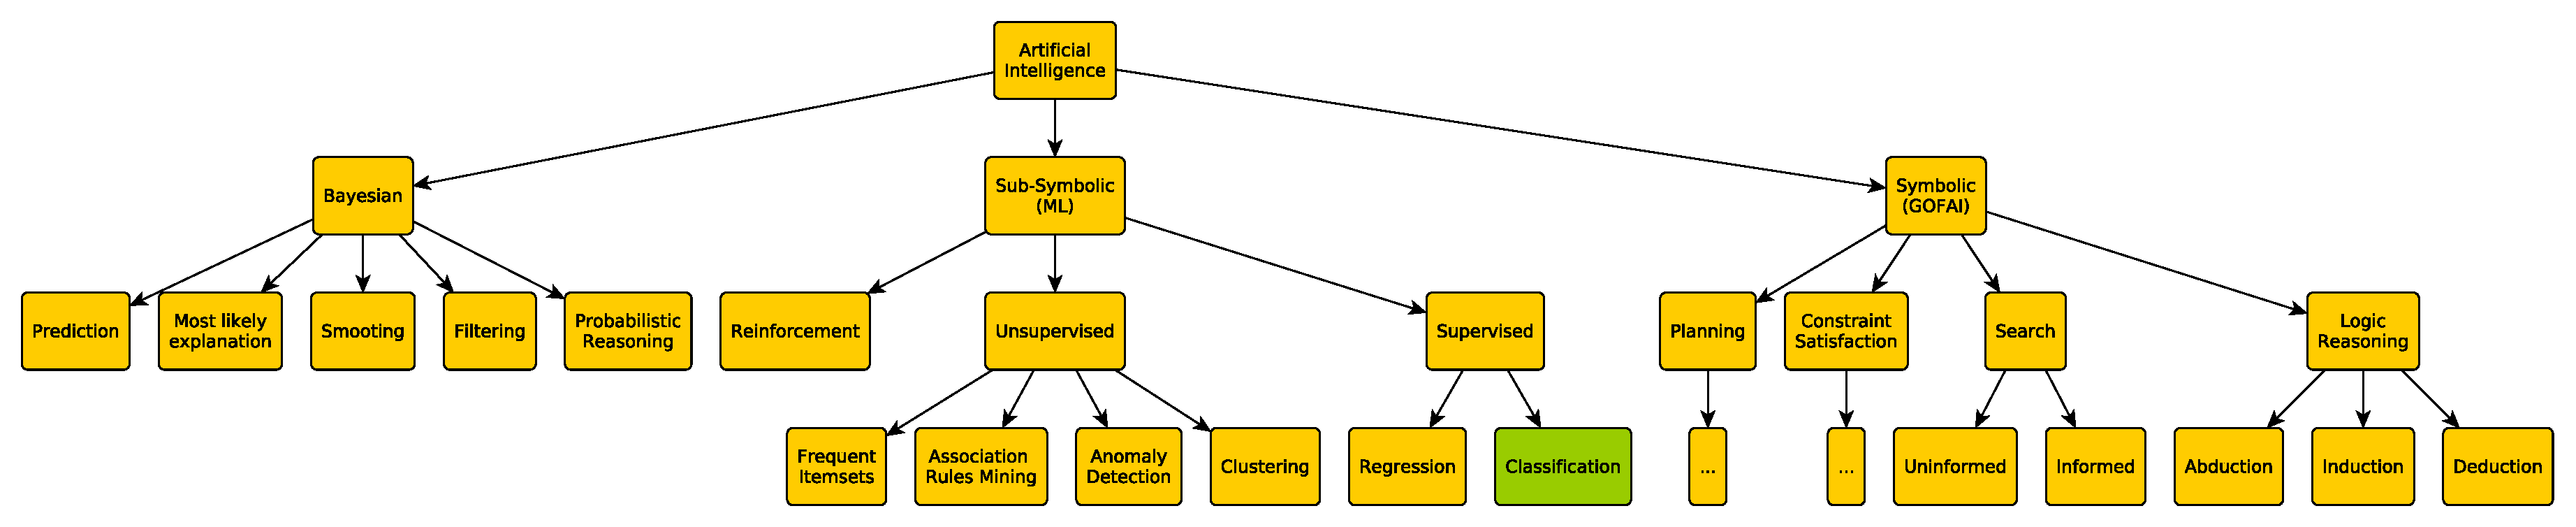
\includegraphics[width=.8\linewidth]{figures/random-image.pdf}
%    \caption{Some random image}
%    \label{fig:random-image}
%\end{figure}

%\section{Some cool topic}

%\chapter{Contribution}

%You may also put some code snippet (which is NOT float by default), eg: \cref{lst:random-code}.

%\lstinputlisting[float,language=Java,label={lst:random-code}]{listings/HelloWorld.java}

%\section{Fancy formulas here}

%----------------------------------------------------------------------------------------
% BIBLIOGRAPHY
%----------------------------------------------------------------------------------------

\backmatter
 
% Remove this as soon as you have the first citation

\bibliographystyle{alpha}
\bibliography{references}

%\begin{acknowledgements} % this is optional
%Optional. Max 1 page.
%\end{acknowledgements}

\end{document}
